
The evaluation of systematic uncertainties in this analysis follows the standard ATLAS Top group recommendations.

Each systematic uncertainty is evaluated at the $1\sigma$ level. The shift is first evaluated at the reconstructed level and then propagated into the unfolding. The result is compared to the spectrum unfolded without a systematic shift. Except where otherwise indicated, individual systematic uncertainties are assumed to be uncorrelated. 

The final \chisq\ conclusions in this analysis rely not just on the bin errors of the final distribution, but on the full covariance matrix. The covariance matrices for systematics are evaluated in one of two ways. Some uncertainties depend on the difference between two discrete spectra (e.g. one generator unfolded against another), and the covariance is taken as the outer product of the systematic uncertainty for each bin. For nuisance parameters such as JES, the full covariance matrix can be computed using pseudoexperiments where the relevant parameter is varied according to a Gaussian probability distribution. The details of these two procedures are given below.

\section{Detector modeling}
Detector modeling uncertainties are evaluated using the baseline \ttbar\ simulation by varying the
default scale factors within their systematic uncertainties. Jet-related uncertainties, primarily the jet energy scale, are the biggest source of detector modeling uncertainity. Uncertainities due to lepton isolation, reconstruction, identification and trigger efficiencies have been evaluated, but found to be negligible. 


%The differences between the varied and nominal unfolded distributions are added in quadrature, symmetrizing if necessary. Finally, the distributions are smoothed with a gaussian kernel procedure to reduce non-physical bin-to-bin fluctuations. 
\subsection{Nuisance parameters}
\label{ss:np}
Jet energy scale uncertainties are evaluated according to the procedure outlined in Reference~\cite{JES}.
Each of the 23 \emph{nuisance parameters} (independent sources of uncertainty) is independently varied.
The jet energy resolution (JER) uncertainty is derived from measurements of the jet response in data and found to agree well with simulation. Jet energy is smeared using
a function that depends on  \pt\ and $\eta$.    Because this procedure only allows for an increase in resolution, 
the resulting uncertainty is symmetrized.
%The systematic uncertainty due to the JVF cut was estimated by varying the JVF with the \texttt{ JVFUncertaintyTool-00-00-04}.
%The jet reconstruction efficiency and its uncertainty were measured in data using the fraction track-jets matched to calorimeter jets.
% The difference between simulation and data is taken as the uncertainty. 
The uncertainty on the jet finding efficiency is evaluated by randomly dropping jets in the nominal simulation
and reanalyzing the resulting data.  The resulting difference is then symmetrized. 


The $b$-tagging scale factor and uncertainty for $b$-tagging efficiency and mistag is also evaluated using results discussed in Reference~\cite{btagpaper}. The modeling of the electron
and muon trigger and identification efficiencies, energy scales and resolutions 
were studied using $Z\rightarrow ee/\mu\mu$, $J/\psi\rightarrow ee/\mu\mu$ and
$W\rightarrow e\nu$ events in data and simulation, using the techniques
described in References \cite{PERF-2013-03,PERF-2013-05,PERF-2014-05}.


\subsection{Computation of uncertainty}
\label{ss:systoy}
The impact of these systematic uncertainties on reconstructed extra jets is evaluated by varying each individual scale factor and reanalyzing the simulated data using the same prescription as for the nominal. The standard ATLAS procedure for evaluating detector systematic uncertainties is to vary each nuisance parameter individually by $\pm 1\sigma$. However, this method does not allow the construction of a full covariance matrix. The procedure used here is similar to that used in Ref.~\cite{Bell:1470588}. A set of 1000 modified samples is constructed from the full statistics of the \powpy\ simulation. For each sample, each nuisance parameter $i$ is varied by $\lambda_i ={\textrm Gauss}(0, \sigma_i)$, where $\sigma_i$ is the nuisance parameter uncertainty. The systematic covariance matrix from these samples is then computed:
\begin{equation}
C_{ij}=\frac{1}{1000} \Sigma_{x=0}^{1000} \left({\mathscr N}_x^i- \left \langle{\mathscr N}^i \right \rangle \right) \left({\mathscr N}_x^j- \left \langle{\mathscr N}^j \right \rangle \right)
\label{eqn:cov}
\end{equation}
where $\left \langle{\mathscr N}^j \right \rangle$ is the average jets in bin $j$ over all samples and ${\mathscr N}_x^j$ is the number of jets in bin $j$ in a single sample $x$. 

As a cross-check, the uncertainities obtained using this procedure are compared to those obtained using the standard ATLAS method for the most signifigant subset of nuisance parameters. Figure~\ref{fig:ToyJES1} shows the uncertainties from the 15 JES eigenstates on the \pt\ for jets of rank=1-4. The band shows the uncertainty obtained from the samples with gaussian variation of all nuisance parameters. The upper and lower lines shows uncertainty from the quadratic sum of the independent variations of each nuisance parameter by $\pm 1 \sigma$. The distribution of samples values has fitted $\mu=1$ and $\sigma$ consistent with the $\pm 1 \sigma$ method.





\begin{figure}
\begin{subfigure}[]{0.45\textwidth}
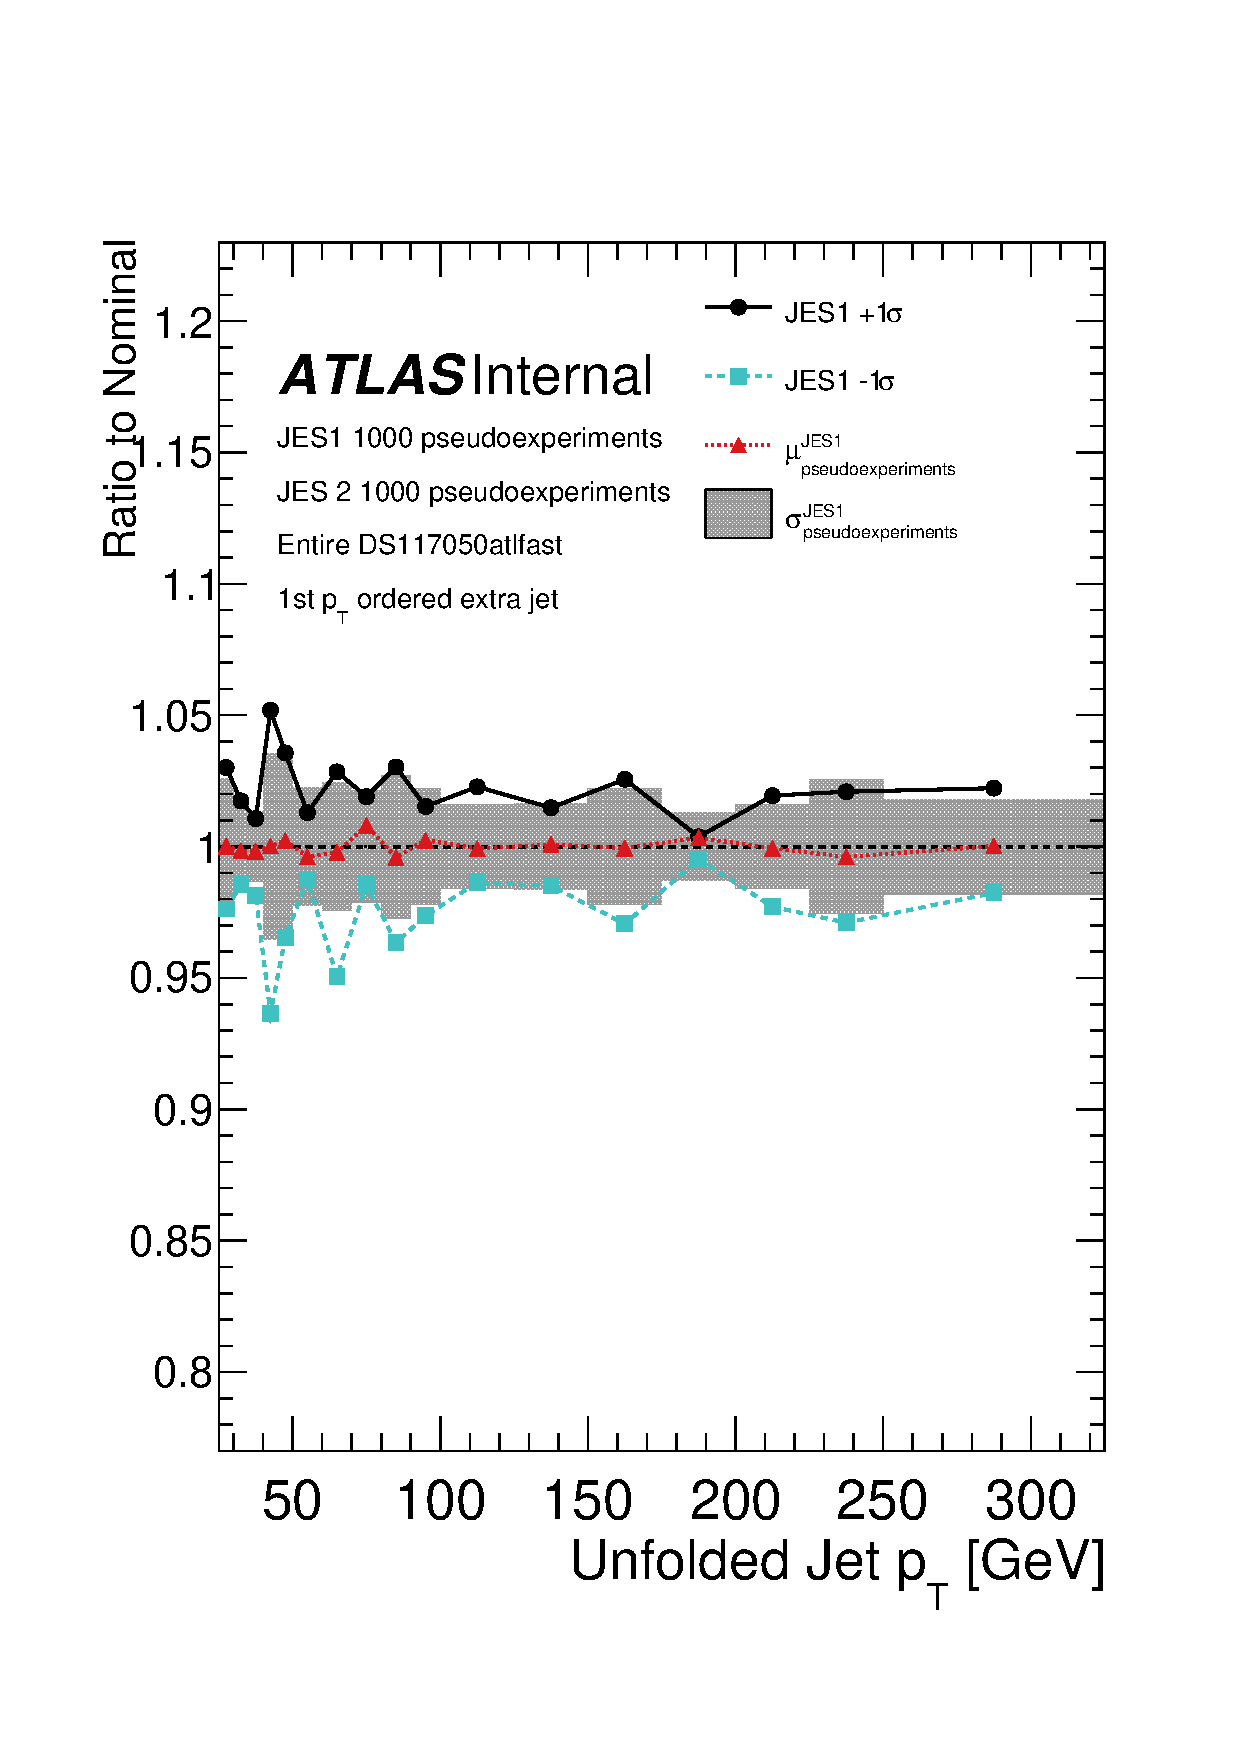
\includegraphics[width=\textwidth]{fig/UnfoldSys/Toy/JES1VarBandRatioJet0.pdf}
\end{subfigure}
\begin{subfigure}[]{0.45\textwidth}
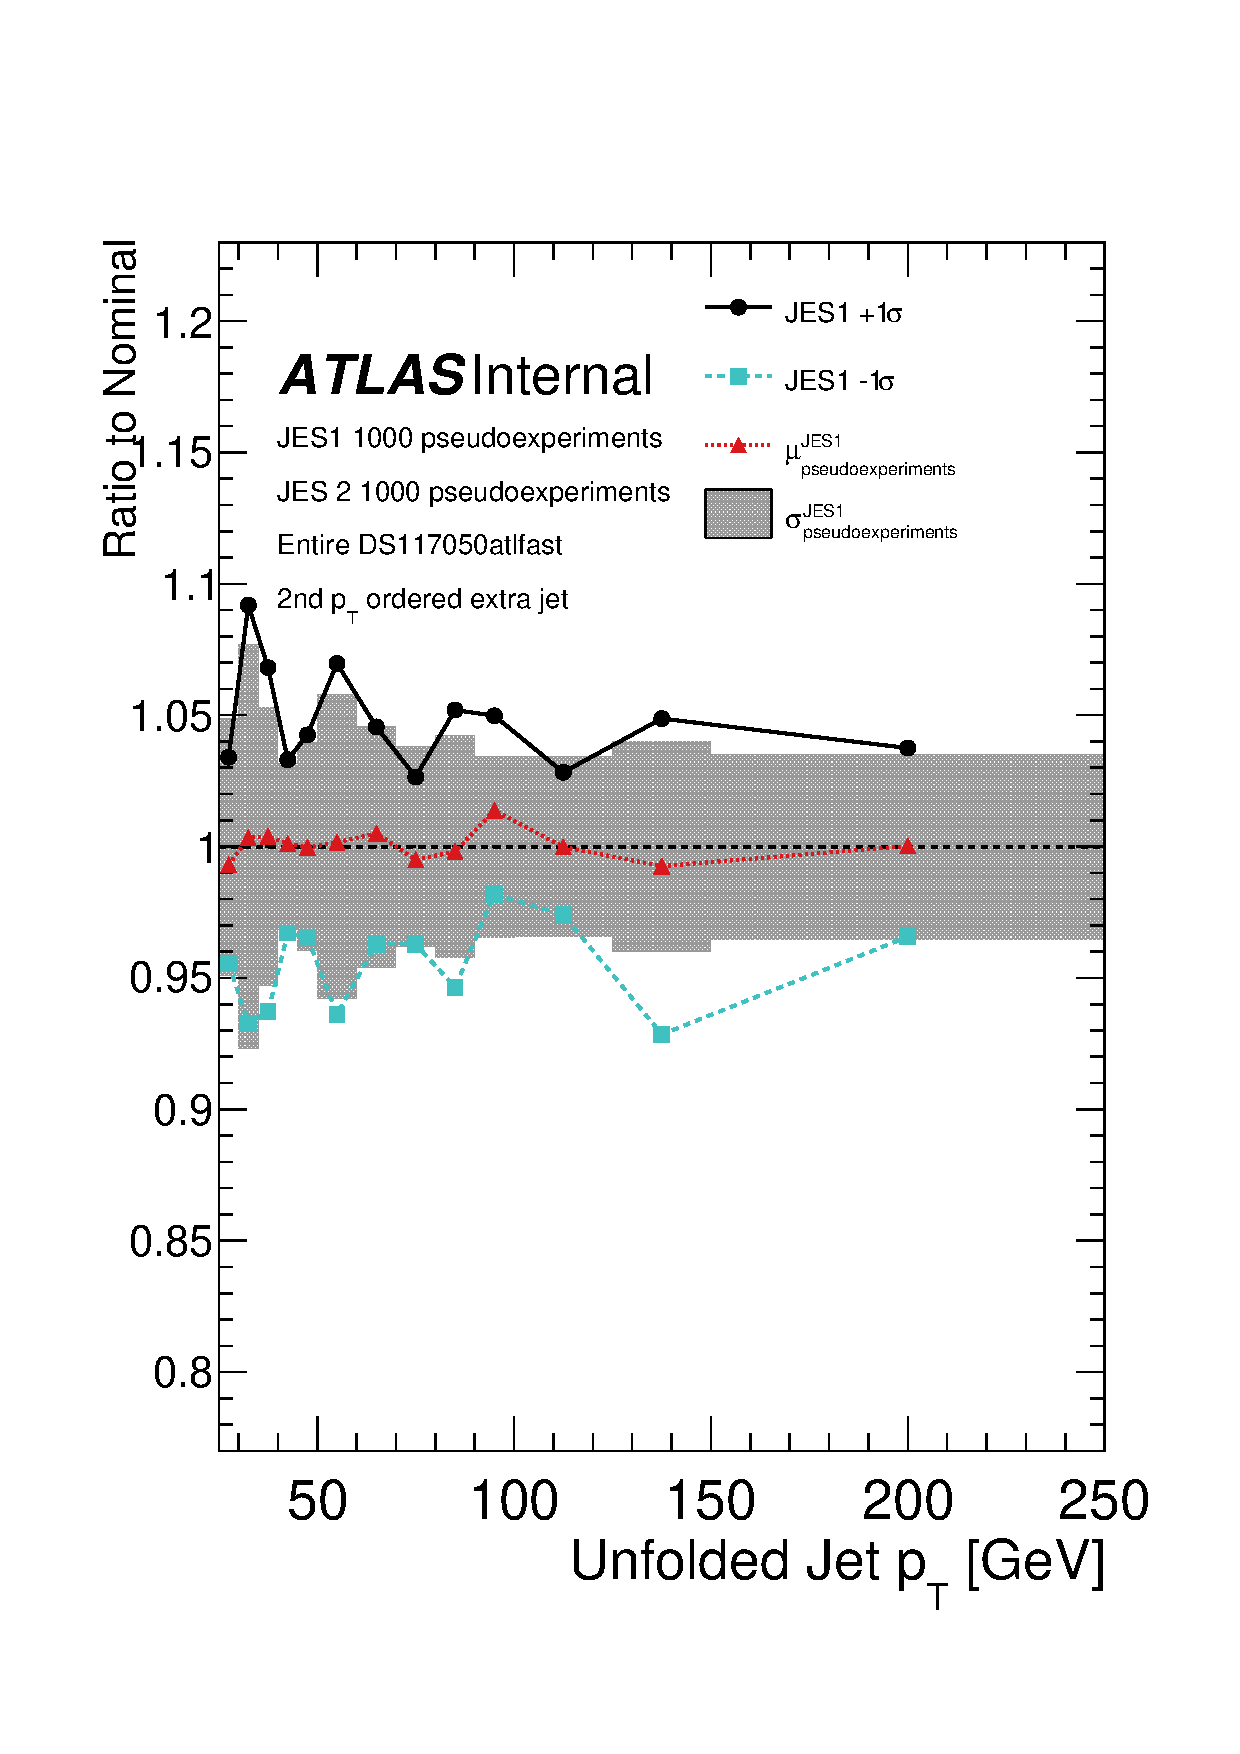
\includegraphics[width=\textwidth]{fig/UnfoldSys/Toy/JES1VarBandRatioJet1.pdf}
\end{subfigure} \\
\begin{subfigure}[]{0.45\textwidth}
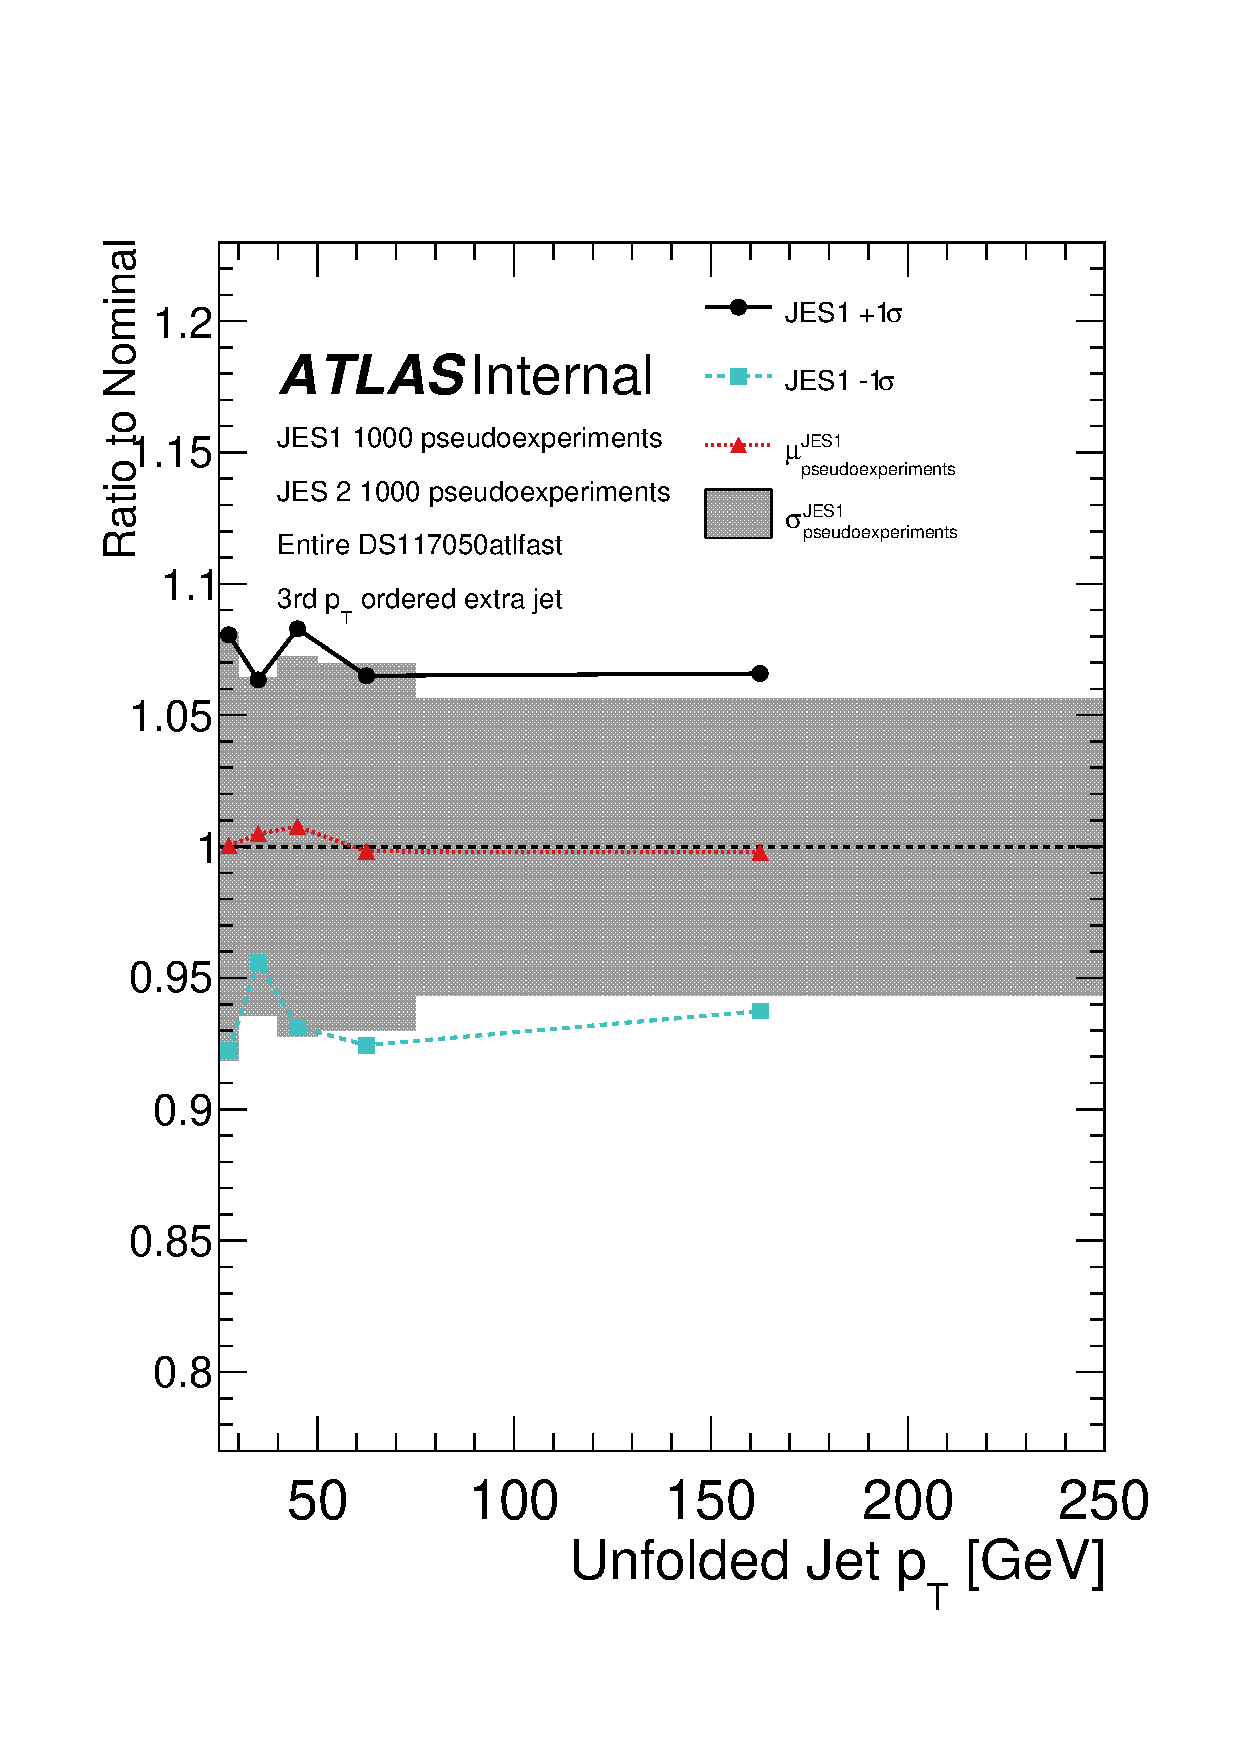
\includegraphics[width=\textwidth]{fig/UnfoldSys/Toy/JES1VarBandRatioJet2.pdf}
\end{subfigure}
\begin{subfigure}[]{0.45\textwidth}
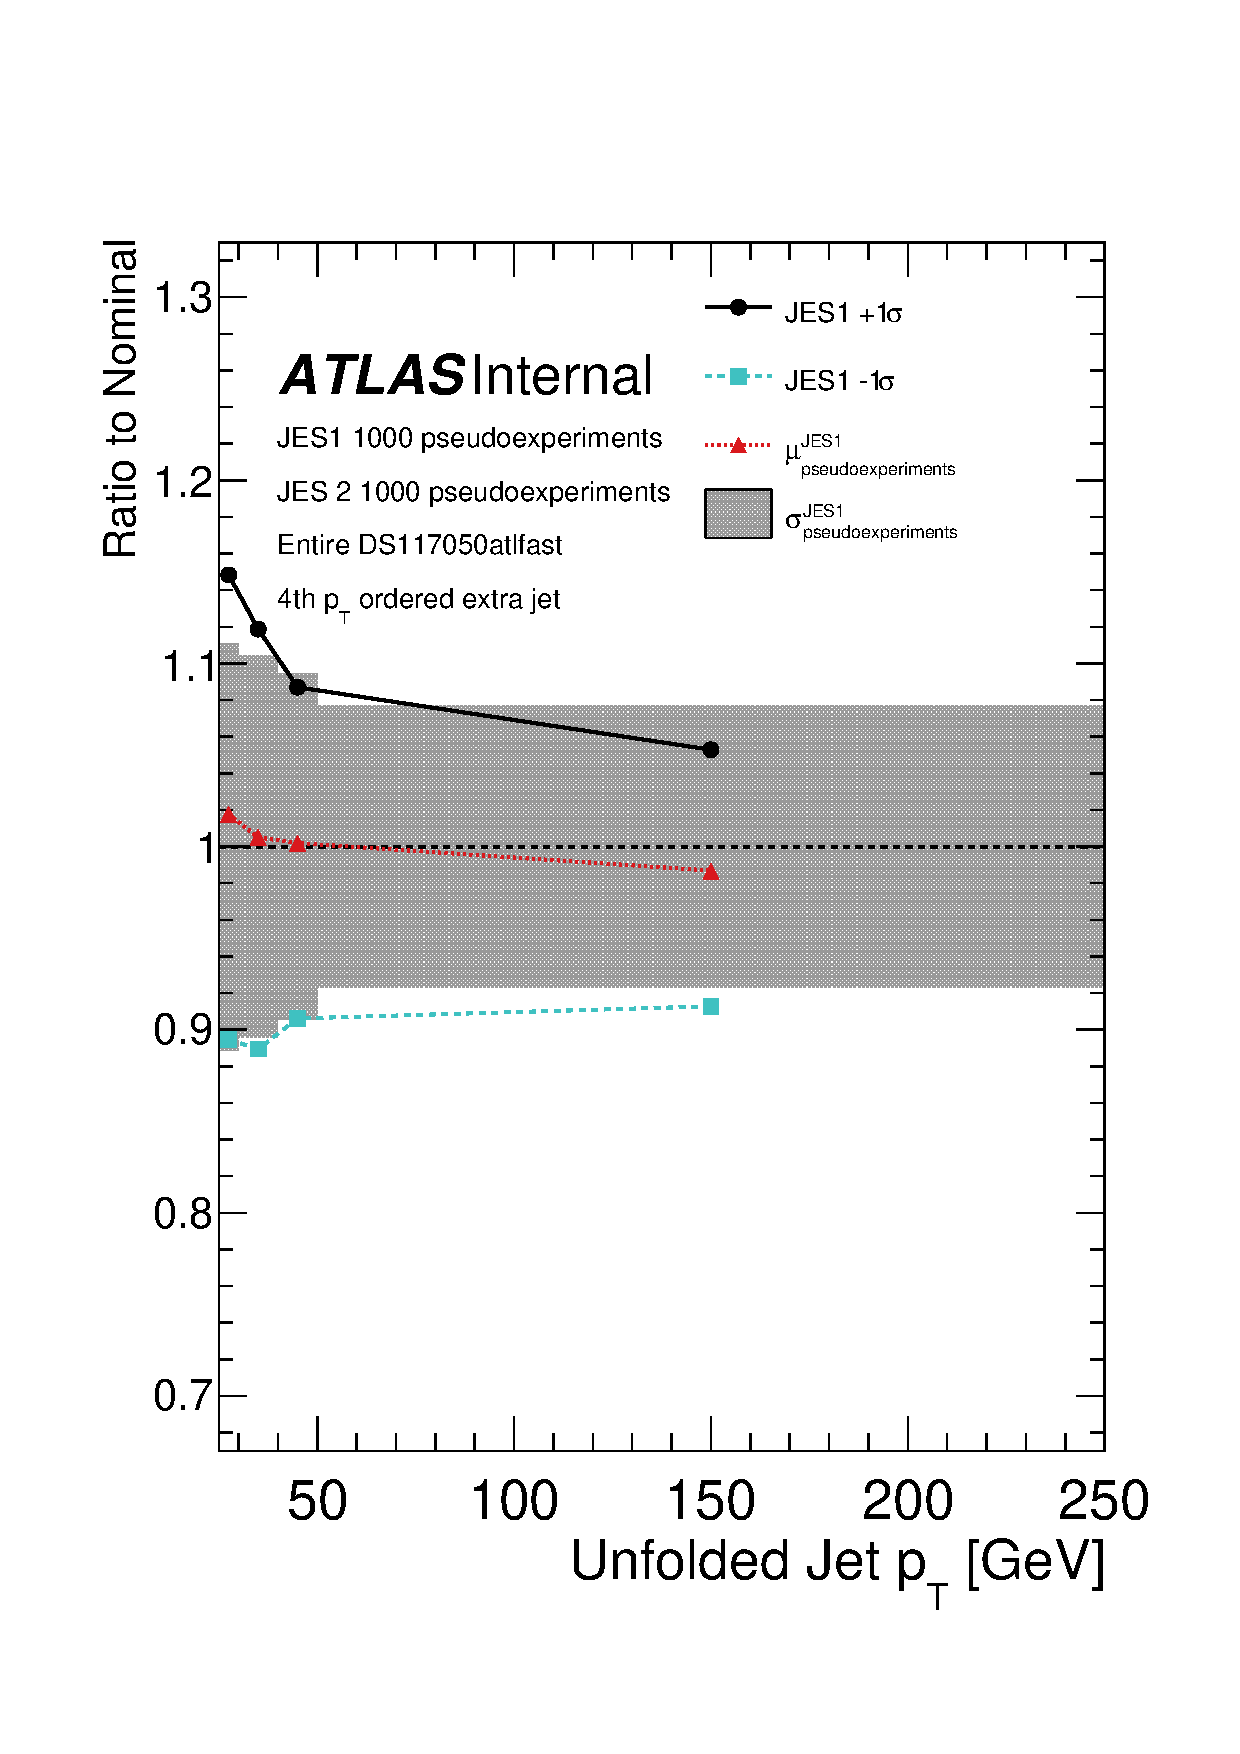
\includegraphics[width=\textwidth]{fig/UnfoldSys/Toy/JES1VarBandRatioJet3.pdf}
\end{subfigure}
\caption{Ratio of reconstructed extra jets spectrum obtained from systematic variations of the 15 JES eigenstate nuisance parameters with respect to that obtained using the nominal parameters. The band shows the uncertainty obtained from the samples with gaussian variation of all nuisance parameters. The upper and lower lines shows uncertainty from the quadratic sum of the independent variations of each nuisance parameter by $\pm 1 \sigma$. The distribution of samples values has fitted $\mu=1$ and $\sigma$ consistent with the $\pm 1 \sigma$ method. }
\label{fig:ToyJES1}
\end{figure}



% \section{Input extra jet spectrum}
% \label{ss:unfsystt}
% %To test whether RooUnfold properly unfolds extra jet spectra that are different from those used to construct the  

% Differences in \ttbar modeling are found to be properly handled by the unfolding procedure, as demonstrated in Section~\ref{ss:stress} and Table~\ref{t:stress}. Thus, the systematic uncertainty due to the input \pt\ spectrum is already included in the (inverse) covariance matrix returned from the unfolding and is not assigned an additional systematic.

\section{Single top rate}
\label{ss:wt}
Since the single top contribution is treated as signal, a systematic uncertainty must be placed on the rate of selected single top events relative to \ttbar.  To assess the uncertainty on the extra jets, the single top rate is varied relative to the baseline 2.9\% computed in Table~\ref{t:sel}. The uncertainty for each bin due to the single top is given by the maximum difference between the baseline 2.9\% single top and 0\% or 5.8\%  single top. The results of this study can be found in Appendix~\ref{app:unfoldwt}.
\begin{displaymath}
\sigma_{ij}\equiv \left \langle \max {|{\mathscr N}_{5.8\%}^i-{\mathscr N}_{2.9\%}^i|, {\mathscr N}_{0\%}^i-{\mathscr N}_{2.9\%}^i|} \right \rangle \left \langle \max {|{\mathscr N}_{5.8\%}^j-{\mathscr N}_{2.9\%}^j|, {\mathscr N}_{0\%}^j-{\mathscr N}_{2.9\%}^j|} \right \rangle
\end{displaymath}

\section{Pileup and false jet background}
\label{ss:sysbkg}
Before unfolding, unmatched jets are subtracted from the measured data distribution. The uncertainty on the modeling of these jets is estimated 
by taking the difference between the pileup and false jets rates obtained in Chapter~\ref{ss:pileup} with the
rate obtained from the baseline \powpy\ simulation.
The unmatched extra jets obtained using these two methods are shown in Figure~\ref{fig:FalseComp}. 
The two distributions agree well at low \pt\ but differ slightly at higher \pt. This systematic uncertainty is small compared to the statistical uncertainty of the samples.
\begin{displaymath}
\sigma_{ij} \equiv \left \langle {\mathscr N}^{i}_{\textrm{false} \textsc{PowHeg+Pythia} }-{\mathscr N}^{i}_{\textrm{ZeroBias~false}} \right \rangle \left \langle {\mathscr N}^{j}_{\textrm{false} \textsc{PowHeg+Pythia} }-{\mathscr N}^{j}_{\textrm{ZeroBias~false}} \right \rangle
\end{displaymath}
\section{Input extra jet spectrum}
\label{ss:unfsystt}
Uncertainty due to the modeling of the input \ttbar\ spectrum for the unfolding is taken from stress tests constructed using the method described in Chapter~\ref{ss:stress}.

Following the prescription outlined by the Top group (see twiki Ref.~\cite{topsys}), the following input generator samples and unfolding procedures are used to evaluate different components of modeling uncertainty:
\begin{description}
\item[NLO generator:] \madpy\ are unfolded using a response matrix and correction factors obtained from \powpy. \madpy\ is used rather than \mcnlohw because \mcnlohw\ is inconsistent with the reconstructed distributions.
\item[Shower:] \pow+\hw\ are unfolded using a response matrix and correction factors obtained from \powpy.
\item[Radiation:] \madpy\ $q^{2}$ up and down are unfolded using a response matrix and correction factors obtained from nominal radiation \madpy.
\end{description}
In all cases, the unfolded result is compared to the truth for the input generator. 
For each component, the uncertainty is expressed as a covariance matrix obtained from the outer product of the biases:

\begin{equation}
\sigma_{ij} \equiv \left \langle {\mathscr N}^{i}_{\textrm{unf}}-{\mathscr N}^{i}_{\textrm{truth}} \right \rangle \left \langle {\mathscr N}^{j}_{\textrm{unf}}-{\mathscr N}^{j}_{\textrm{truth}} \right \rangle
\end{equation}

The radiation uncertainty is taken from the average bias for \madpy\ $q^{2}$ up and down.

\section{Statistical uncertainty on migration matrix}
\label{ss:mcstats}
As shown in the Figure~\ref{f:res}(a), the migration matrix has some elements far from the diagonal with very few entries. To account for the uncertainty introduced by the migration matrix statistics, pseudoexperiments are unfolded varying the response matrix while keeping the input spectrum constant. The migration matrix, input spectrum and correction factors are all taken from the baseline \powpy\ sample. The contribution to the covariance matrix from this componenet is evaluated according to Equation~\ref{eqn:cov}.

\section{PDF modeling uncertainty}
\label{ss:pdf}
Uncertainty in the modeling of the parton distribution function (PDF) can affect modeling of the extra jets. Following the prescription given in Ref.~\cite{toppdf}, events are reweighted according to the $x$ and $Q^2$ of the corresponding PDF variation. PDF variations are taken from the \mcnlohw\ sample is used 
with 52 variations for the CT10 PDF, 40 variations for the MSTW PDF, and 100 variations for the NNPDF~\footnote{Though \mcnlohw\ shows poor agreement with data, it is the only sample for which $x$ and $Q$ are properly recorded in ATLAS simulation}. 

Each variation is unfolded with the nominal \mcnlohw\ migration matrix. For each bin, the average bias of the variations with respect to the input spectrum is computed. The outer product of these biases is used to compute the covariance for the PDF uncertainty:

\begin{displaymath}
\sigma_{ij} \equiv \left \langle {\mathscr N}^{i}_{\textrm{unf}}-{\mathscr N}^{i}_{\textrm{truth}} \right \rangle \left \langle {\mathscr N}^{j}_{\textrm{unf}}-{\mathscr N}^{j}_{\textrm{truth}} \right \rangle
\end{displaymath}

\begin{figure}
\begin{subfigure}[]{0.45\textwidth}
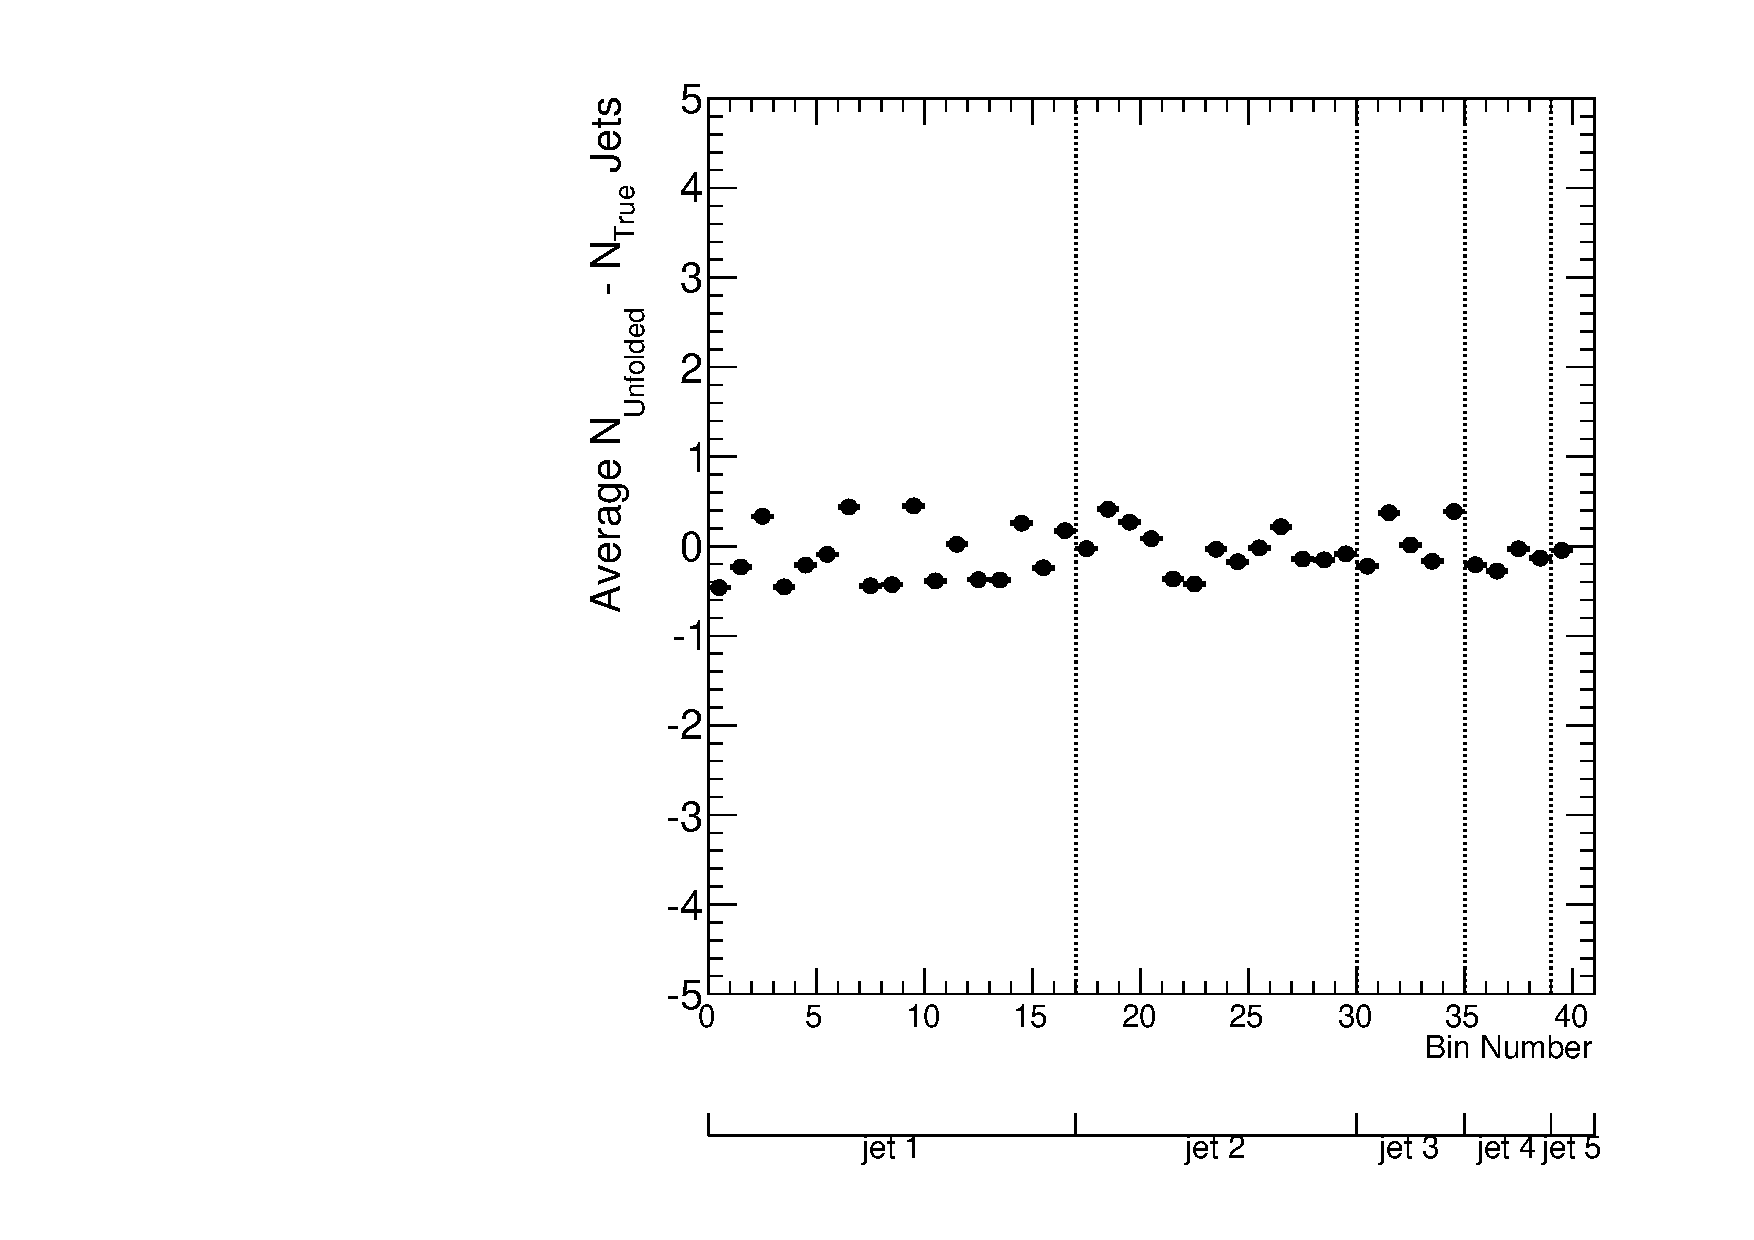
\includegraphics[width=\textwidth]{fig/PDF/AvgBias.pdf}
\end{subfigure}
~
\begin{subfigure}[]{0.45\textwidth}
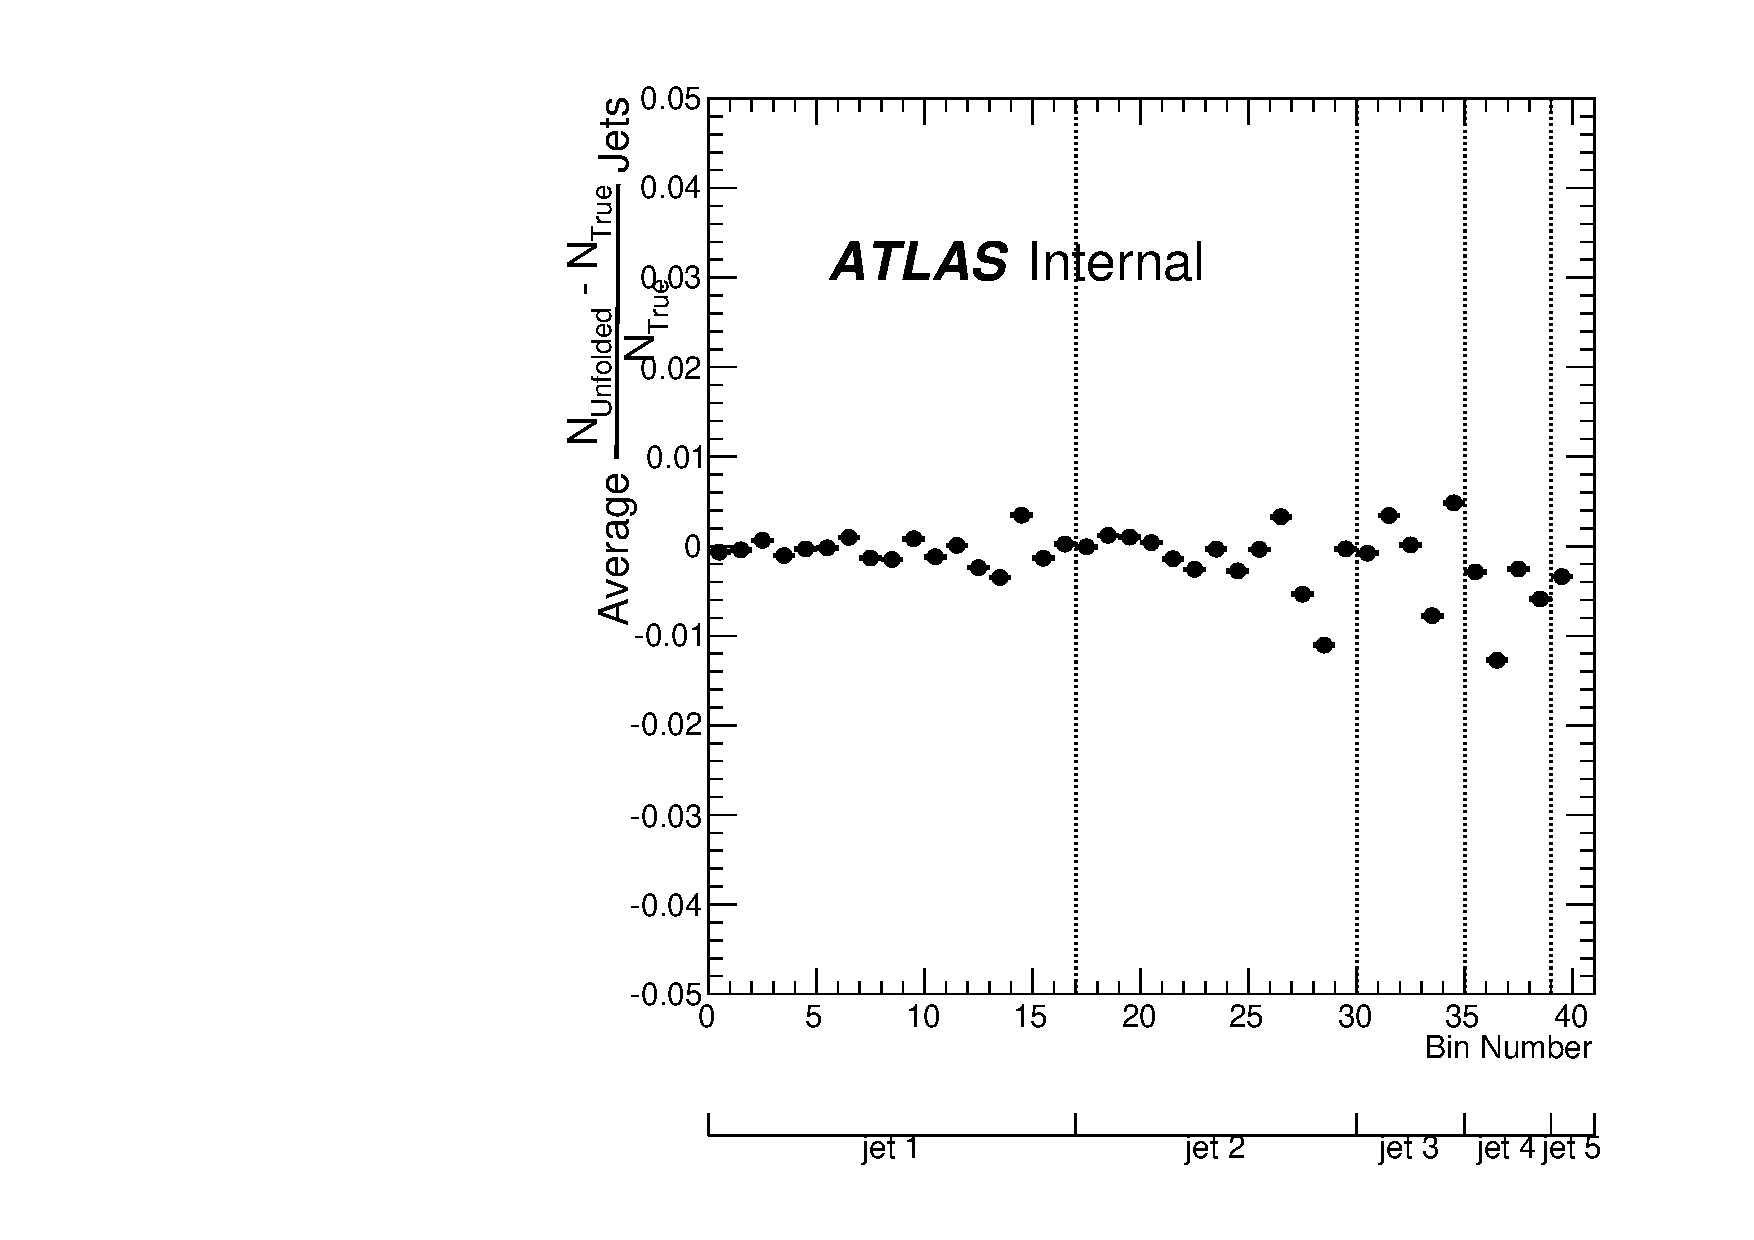
\includegraphics[width=\textwidth]{fig/PDF/AvgFracBias.pdf}
\end{subfigure}
~
\label{fig:pdfbias}
\caption{
(a) bias and (b) fractional bias distributions PDF variations of \mcnlohw unfolded with the nominal \mcnlohw migration matrix. Each bin of the distribution over the pseudoexperiments is fit with a gaussian. The outer product of the bias is used to compute the uncertainty due to the PDF.}
\end{figure}


\begin{figure}
\begin{subfigure}[]{0.45\textwidth}
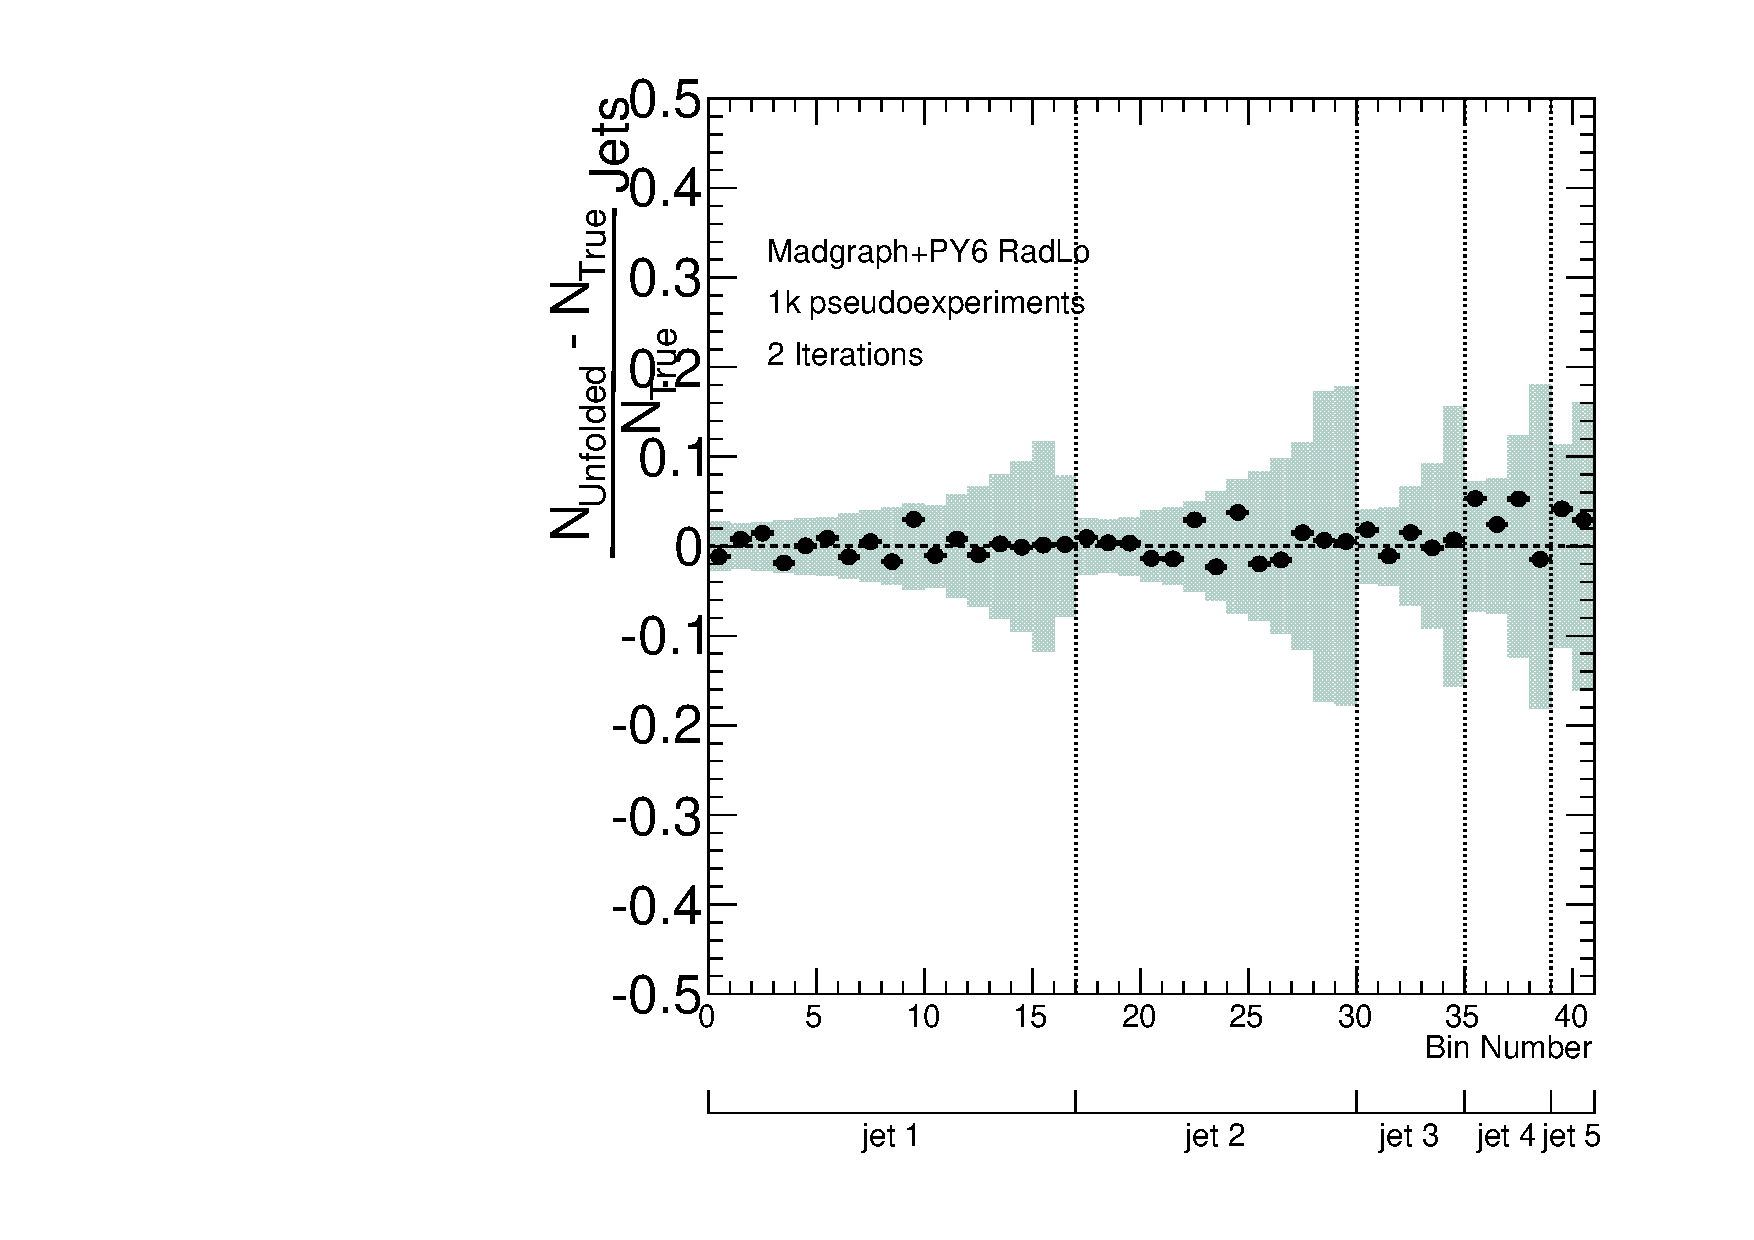
\includegraphics[width=\textwidth]{fig/Stress/110875atlfast/FracBias2Iterations.pdf}
\end{subfigure}
~
\begin{subfigure}[]{0.45\textwidth}
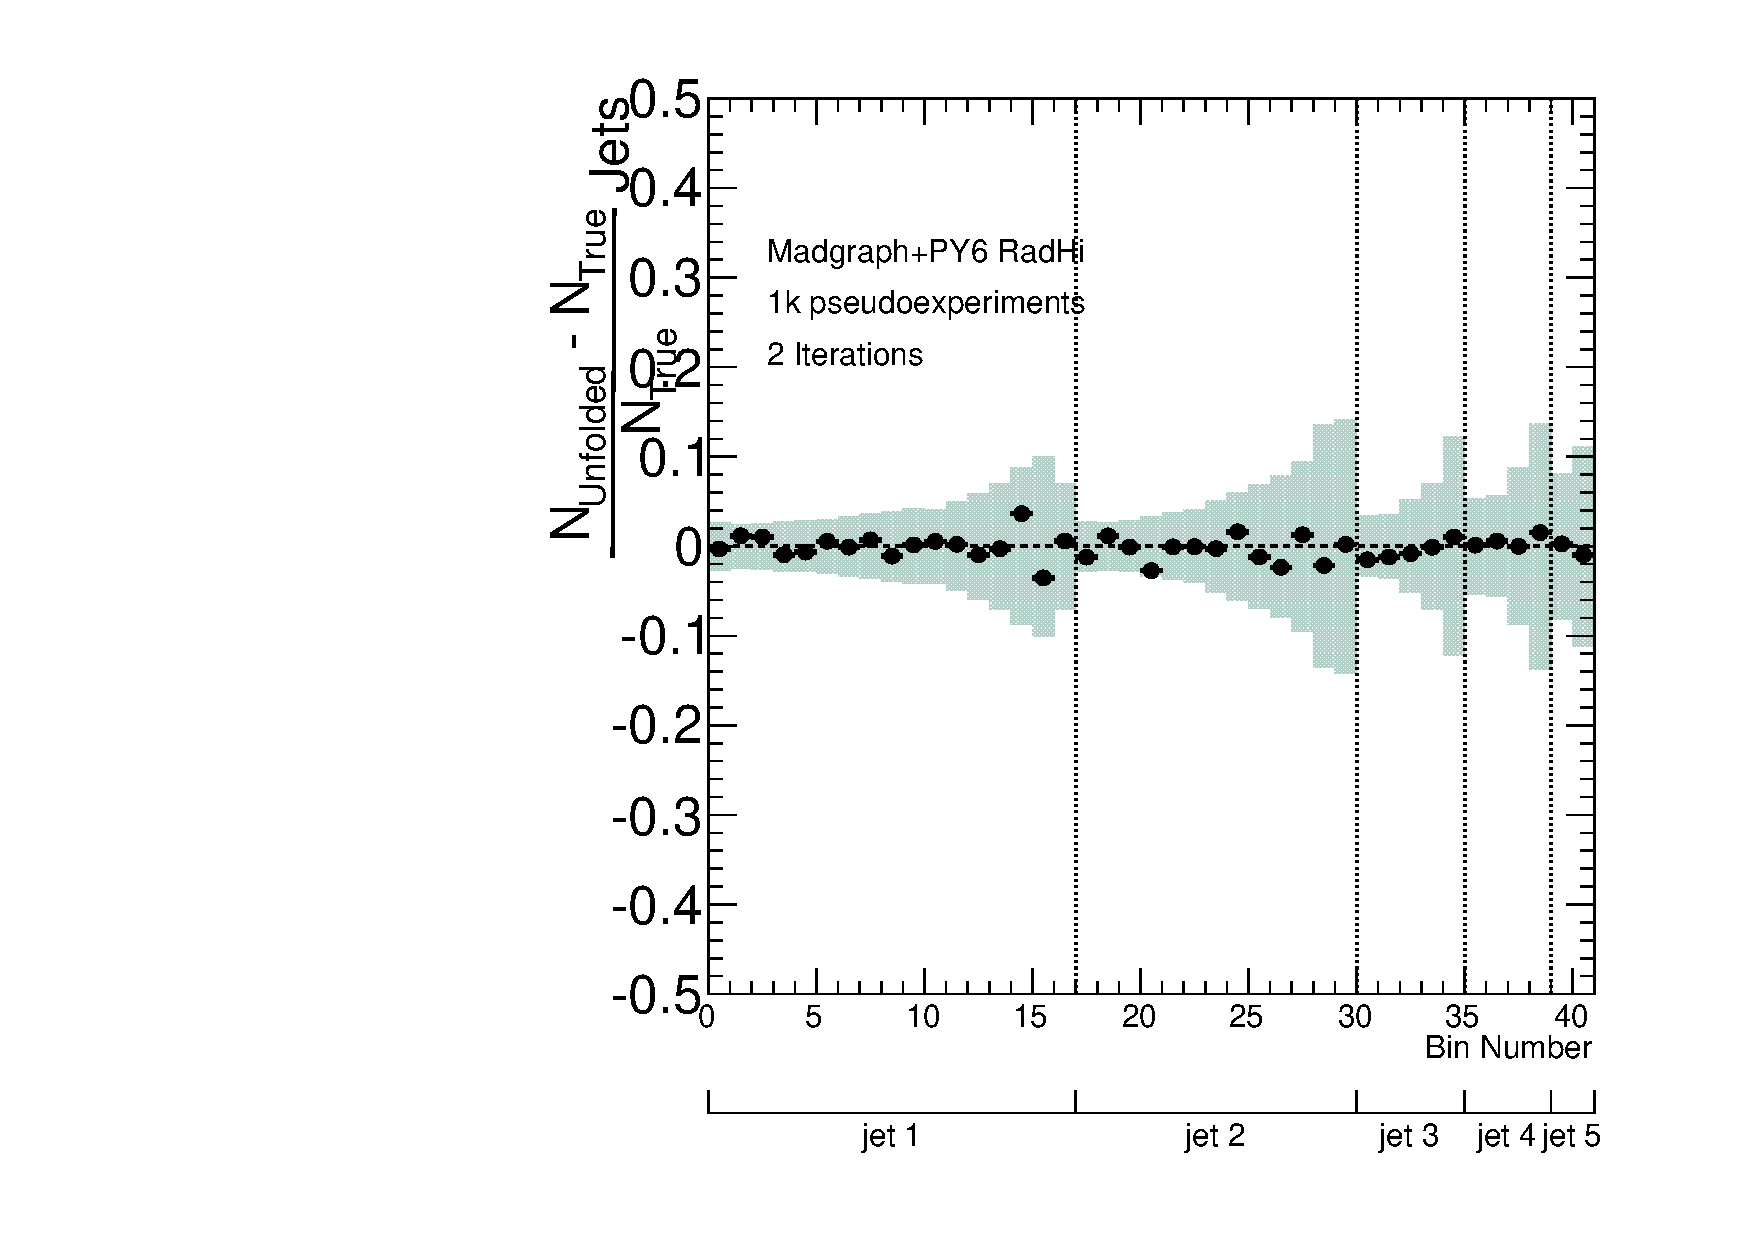
\includegraphics[width=\textwidth]{fig/Stress/110878atlfast/FracBias2Iterations.pdf}
\end{subfigure}
\label{fig:radbias}
\caption{
Fractional bias distributions for pseudoexperiments from \madpy\ radiation samples unfolded against a matrix filled with nominal \madpy. The truth spectrum of the baseline sample is reweighted to match jet \pt\ and multiplicity spectra of (a) \madpy\ RadLo (b) \madpy\ RadHi simulation. One thousand pseudoexperiments, each the size of the events in data, are constructed for each generator and unfolded. The Bayesian unfolding method with 2 iterations is used. Each bin of the distribution over the pseudoexperiments is fit with a gaussian. The black points show the fitted mean of each bin and the blue band shows the fitted sigma.}
\end{figure}


\begin{figure}
~
\begin{subfigure}[]{0.45\textwidth}
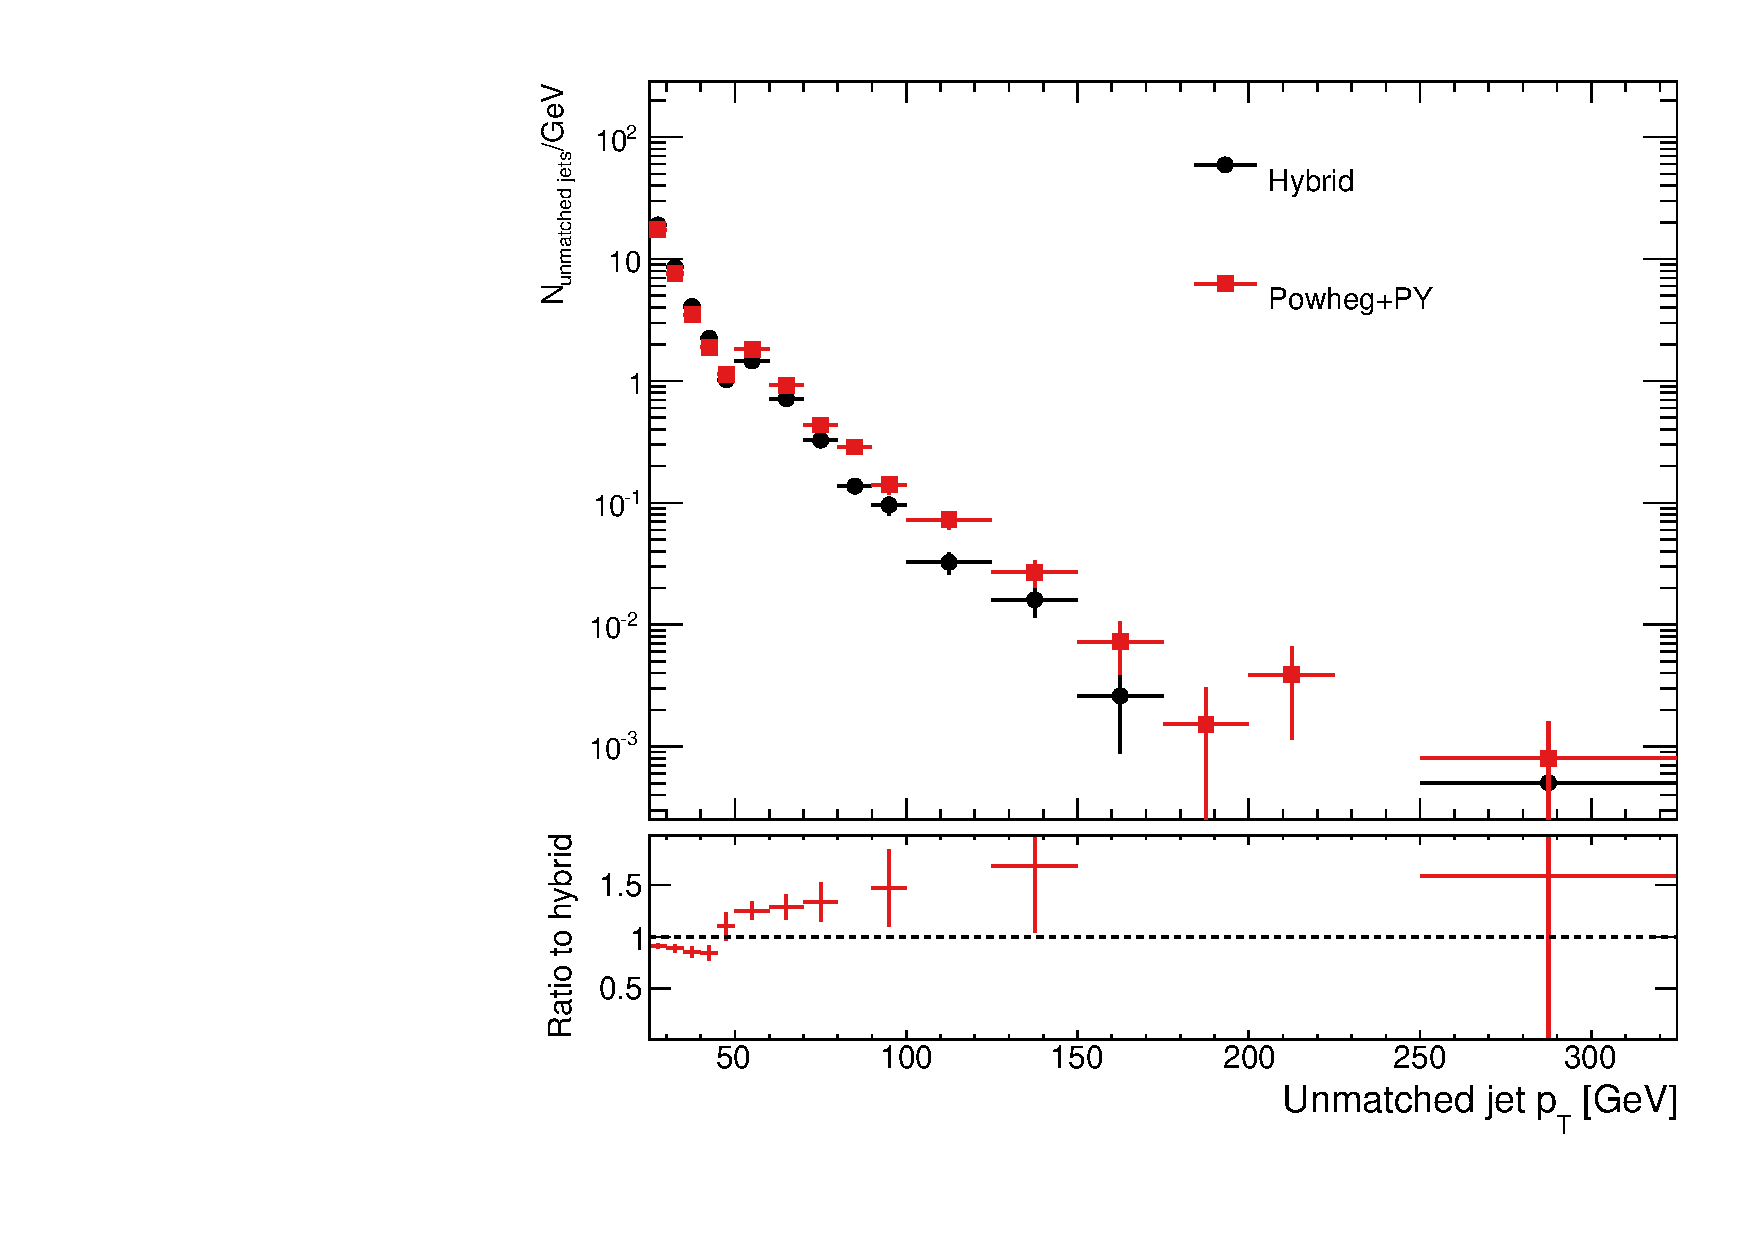
\includegraphics[width=\textwidth]{fig/Pileup/RecoPtFalseJet0.pdf}
\end{subfigure}
~
\begin{subfigure}[]{0.45\textwidth}
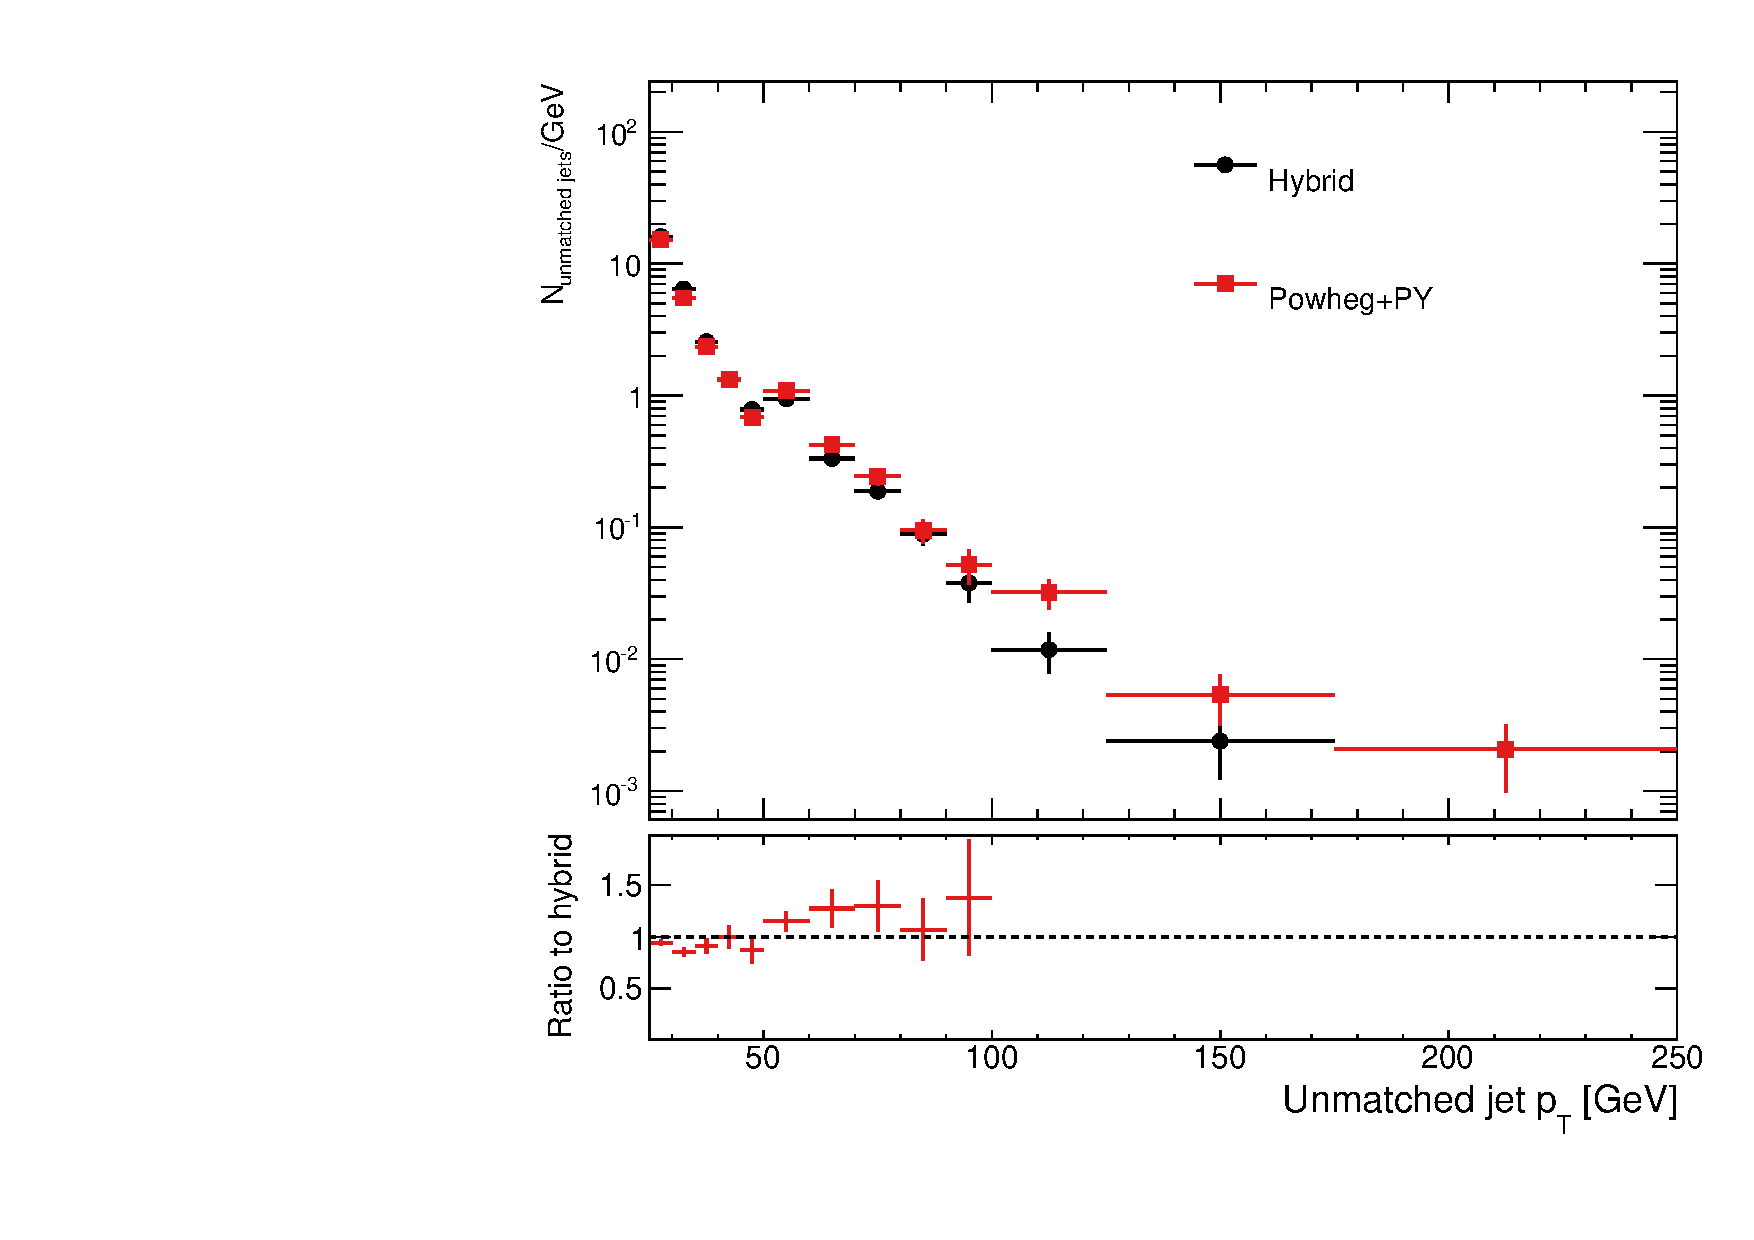
\includegraphics[width=\textwidth]{fig/Pileup/RecoPtFalseJet1.pdf}
\end{subfigure}\\
~
\begin{subfigure}[]{0.45\textwidth}
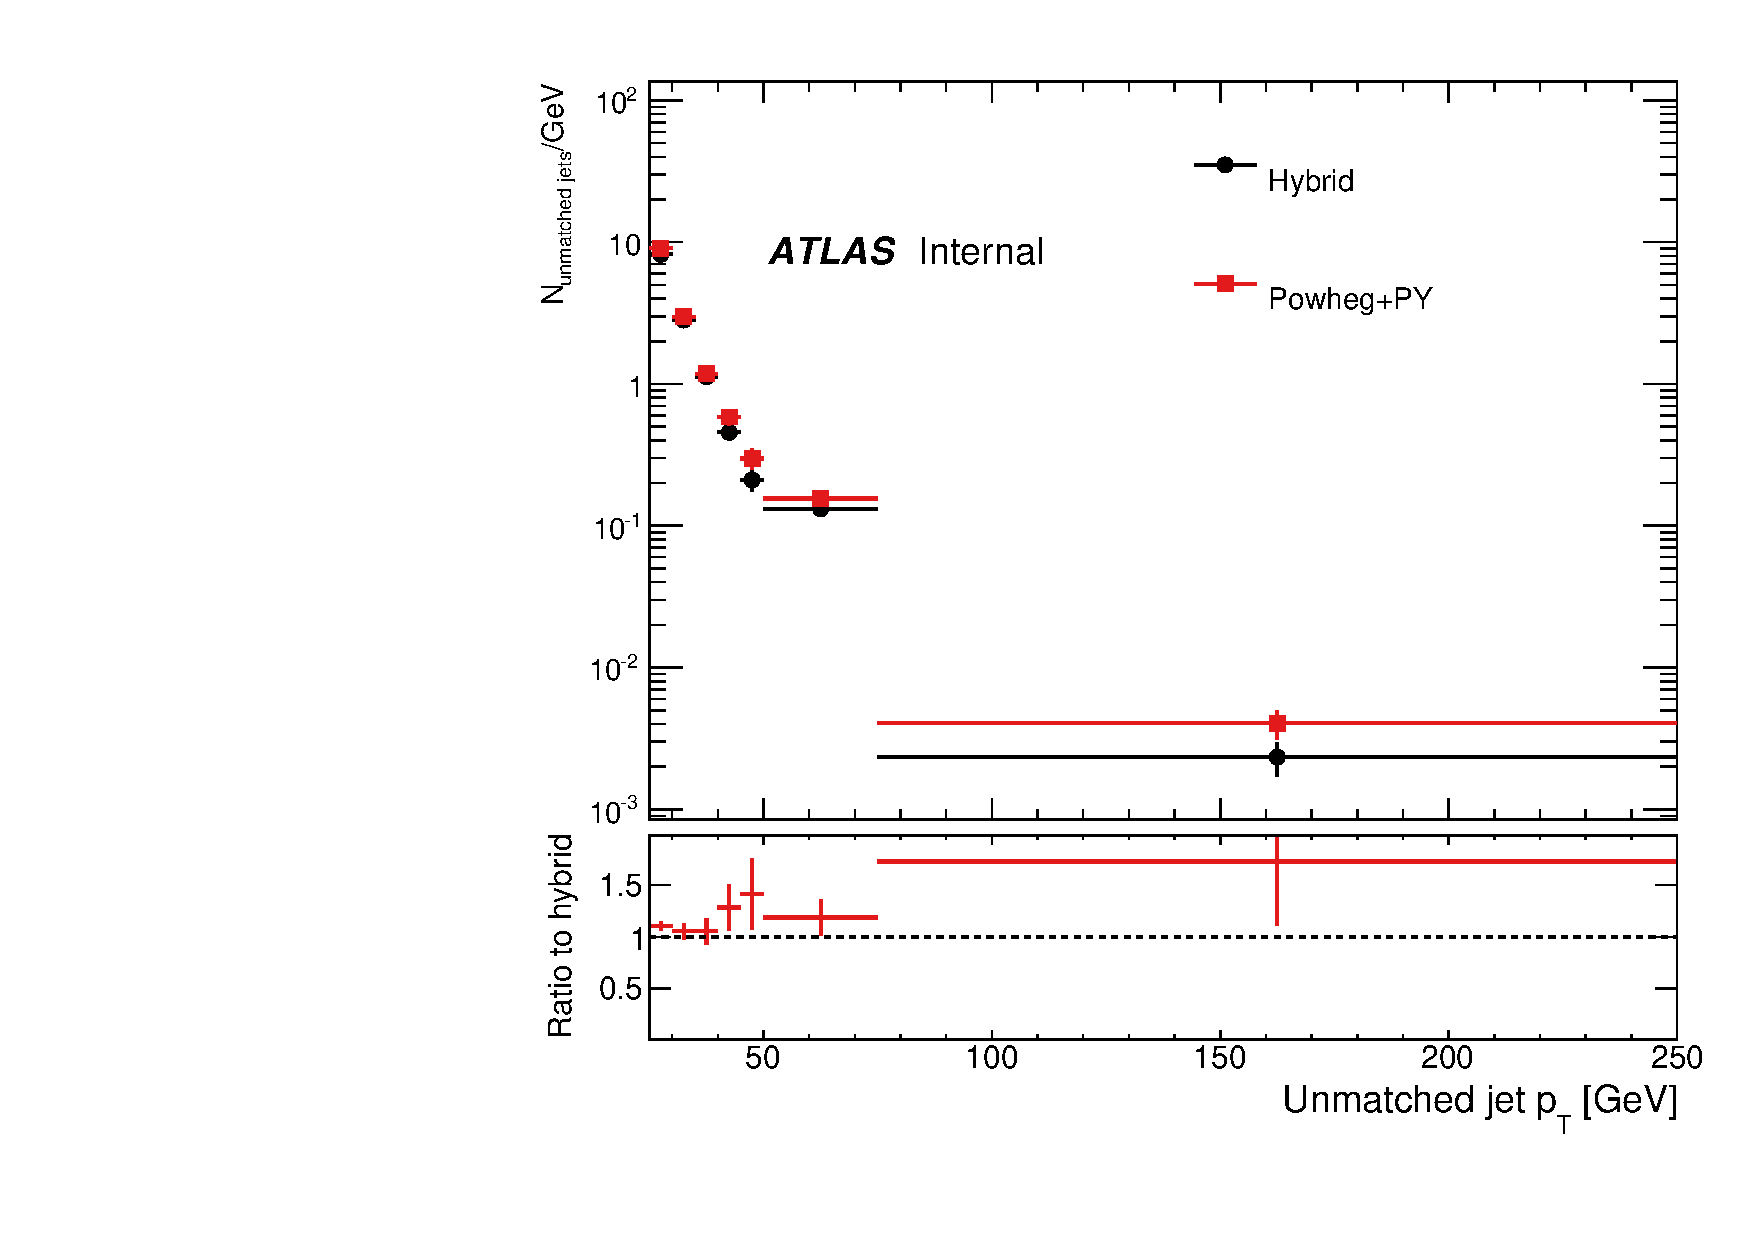
\includegraphics[width=\textwidth]{fig/Pileup/RecoPtFalseJet2.pdf}
\end{subfigure}
~
\begin{subfigure}[]{0.45\textwidth}
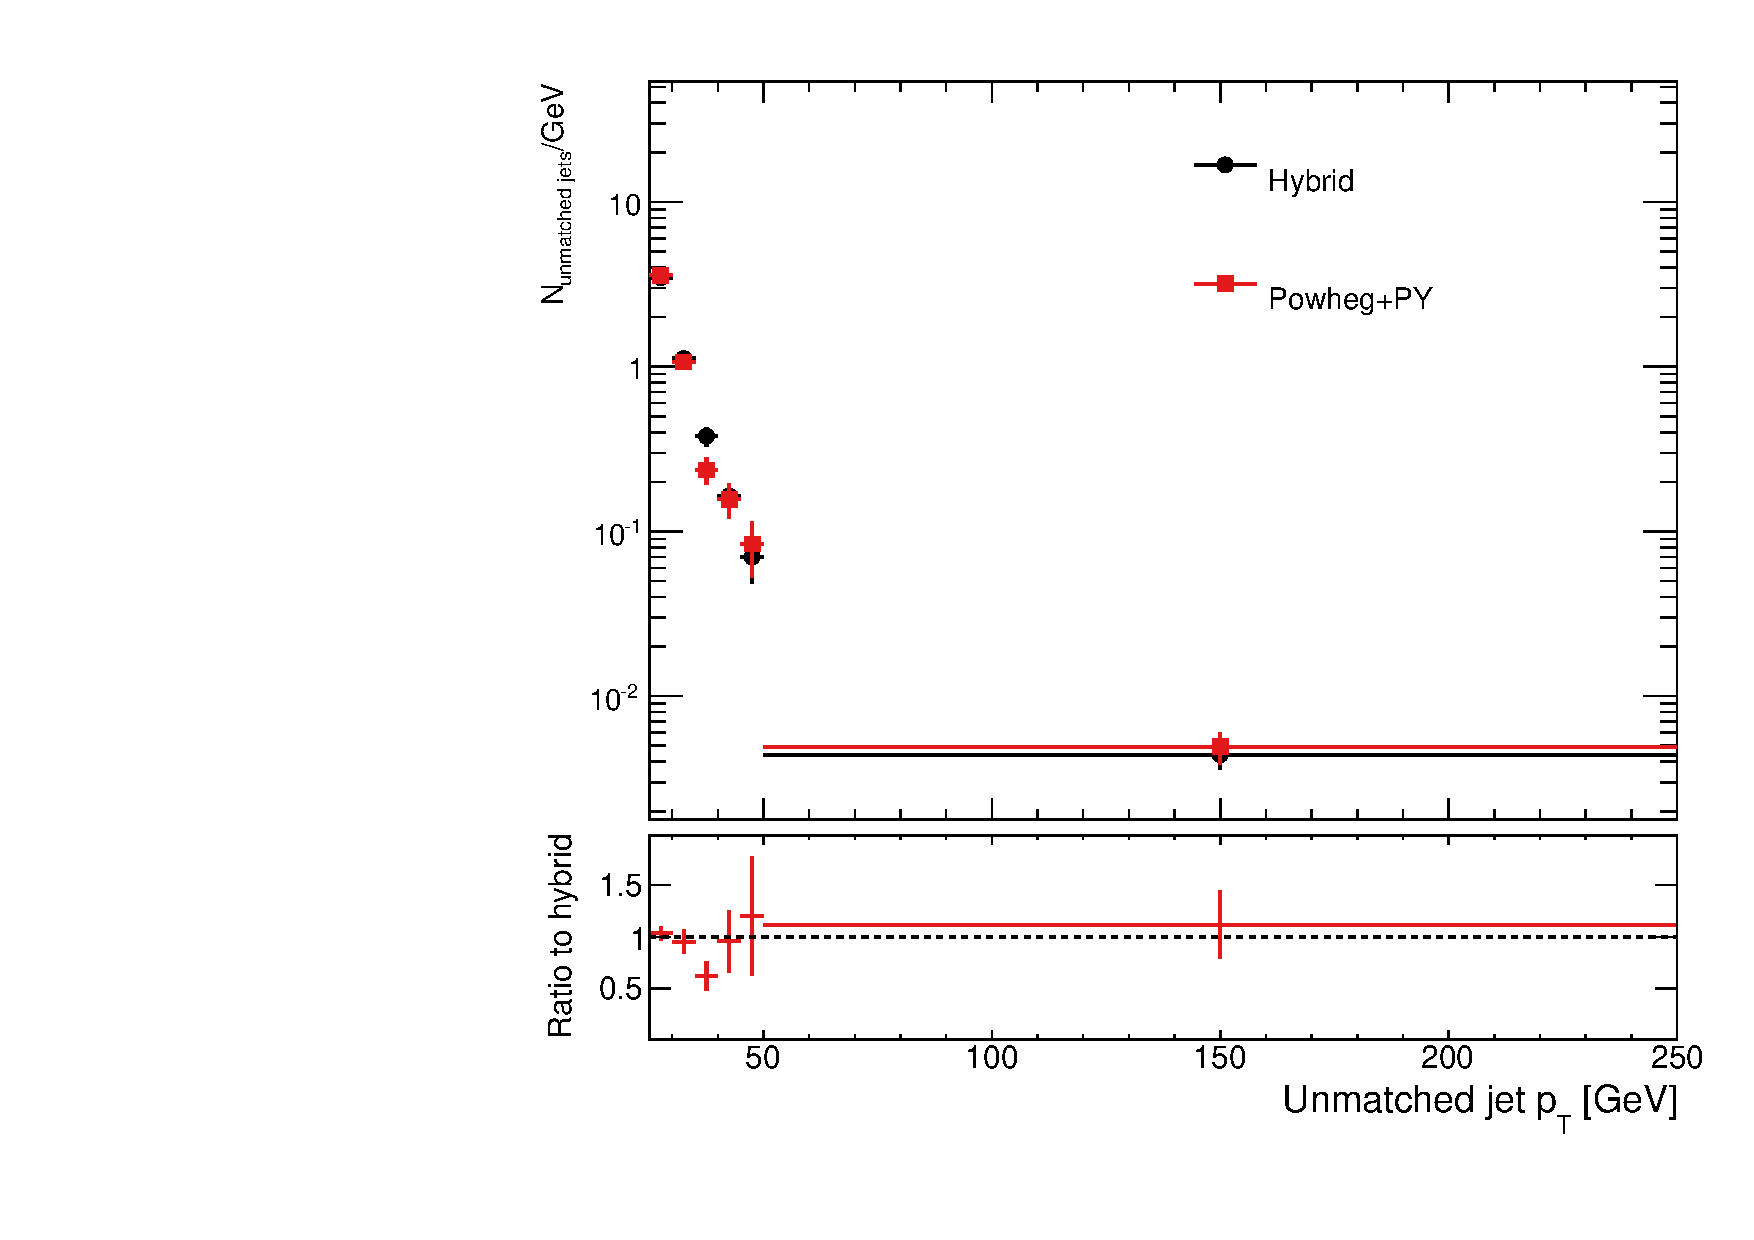
\includegraphics[width=\textwidth]{fig/Pileup/RecoPtFalseJet3.pdf}
\end{subfigure}
~
\caption{Unmatched jets in the baseline \ttbar\ simulation and the hybrid sample. The difference between the two is used to estimate the uncertainty.}
\label{fig:FalseComp}
\end{figure}

\section{Combined uncertainty}
%%%%%SHOULD THIS SECTION MOVE????
A covariance matrix associated with the statistical uncertainty of the input data spectrum is returned from \texttt{RooUnfold}. The covariance matrix due to all sources of uncertainty described above is then added to the \texttt{ RooUnfold} matrix to obtain the final uncertainty on the corrected data. Figure~\ref{fig:cov}  shows (a) the statistical covariance matrix  and (b) total covariance matrix for the unfolded data. The diagonal elements of total matrix are used to obtain uncertainties on unfolded data in bins of \pt\ and rank. The entire matrix is used to assess the agreement between data and generators. 

Figure ~\ref{fig:SmoothSys} shows the sum of uncertainties from all sources, broken into categories as follows.
\begin{description}
\item[Data Statistics:] Statistical uncertainty on the data is returned from \texttt{ RooUnfold}
\item[\ttbar\ modeling:] NLO generator, radiation, and parton shower uncertainties(Chapter~\ref{ss:unfsystt})
\item[MC Stats:] Migration matrix statistics uncertainties (Chapter~\ref{ss:mcstats})
\item[PDF:] PDF variations, determined from \mcnlohw (Chapter~\ref{ss:pdf})
\item[JVF/Unmatched Jets:] Uncertainties from JVF nuisance parameters (Chapter~\ref{ss:np}) and false jet modeling (Chapter~\ref{ss:sysbkg})
\item[JES:] Jet energy scale nuisance parameters (Chapter~\ref{ss:np})
\item[JER/JEFF:] Jet energy resolution and jet finding efficiency nuisance parameters (Chapter~\ref{ss:np})
\item[Other detector:] Lepton and $b$-tag nuisance parameters not in the JES, JER/JEFF or pileup category.
\item[Backgrounds:] Single top rate uncertainty $Wt$ (Chapter\ref{ss:wt}) 
\end{description}

In most bins, statistical uncertainty dominates. At low jet \pt, JES is the largest source of uncertainty. Modeling is the largest source of uncertainty at high jet \pt.


%ADD FIGS AND REFERENCES


% \section{Propagation of uncertainties to multiplicity distributions}
% Statistical uncertainties from RooUnfold and systematic uncertainties from the above procedures are calculated in bins of jet \pt\ and rank. In order to derive the multiplicity from these distributions, the uncertainties must be propagated as a multinomial distribution with a full covariance matrix. Details of this propagation are provided in Appendix~\ref{app:stats}. Pull distributions obtained from pseudoexperiments are shown in Figure~\ref{fig:multpull} and indicate that this calculation overestimates the statistical uncertainty. As recommended by the statistics committee, the final uncertainty on the multiplicity is obtained using the pseudoexperiments.
\begin{figure}
\begin{subfigure}[]{0.45\textwidth}
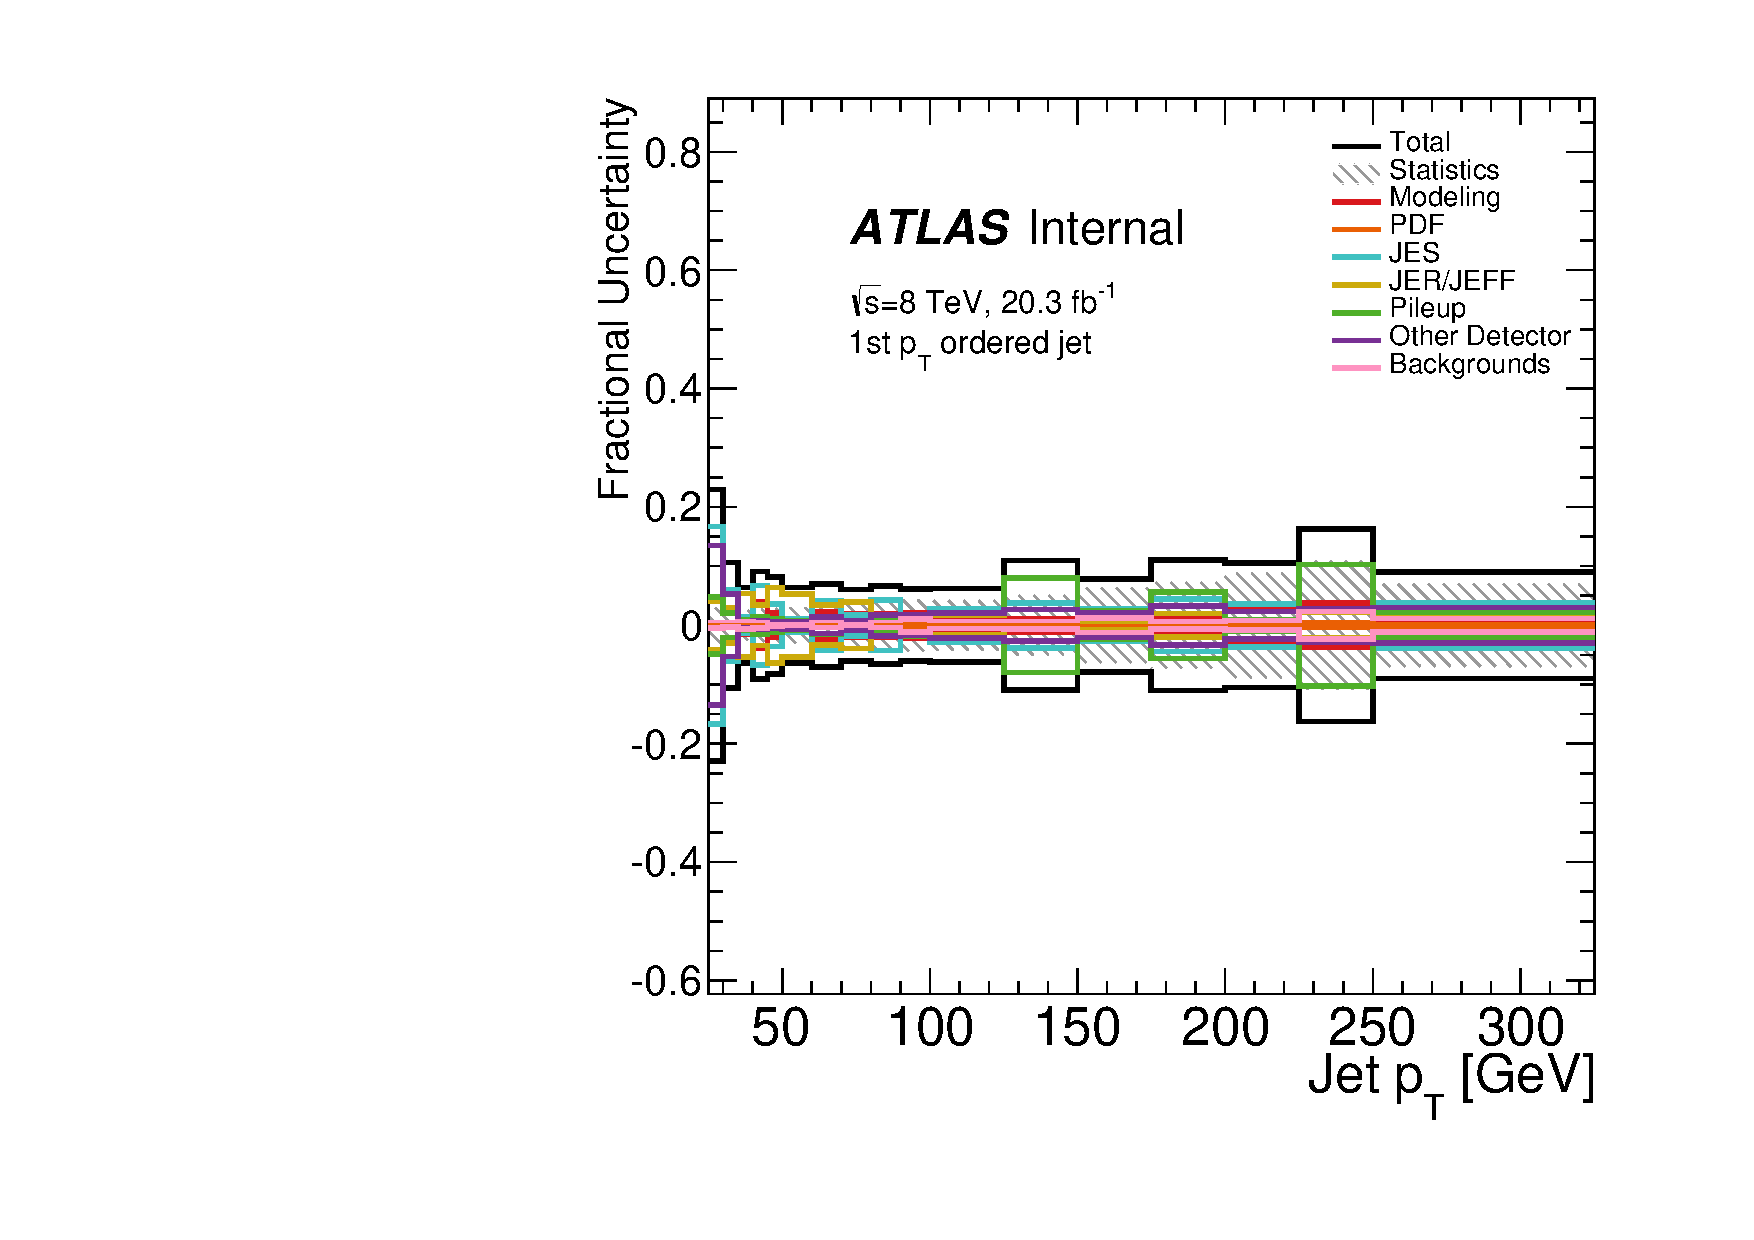
\includegraphics[width=\textwidth]{fig/UnfoldSys/Jet0.pdf}
\end{subfigure}
~
\begin{subfigure}[]{0.45\textwidth}
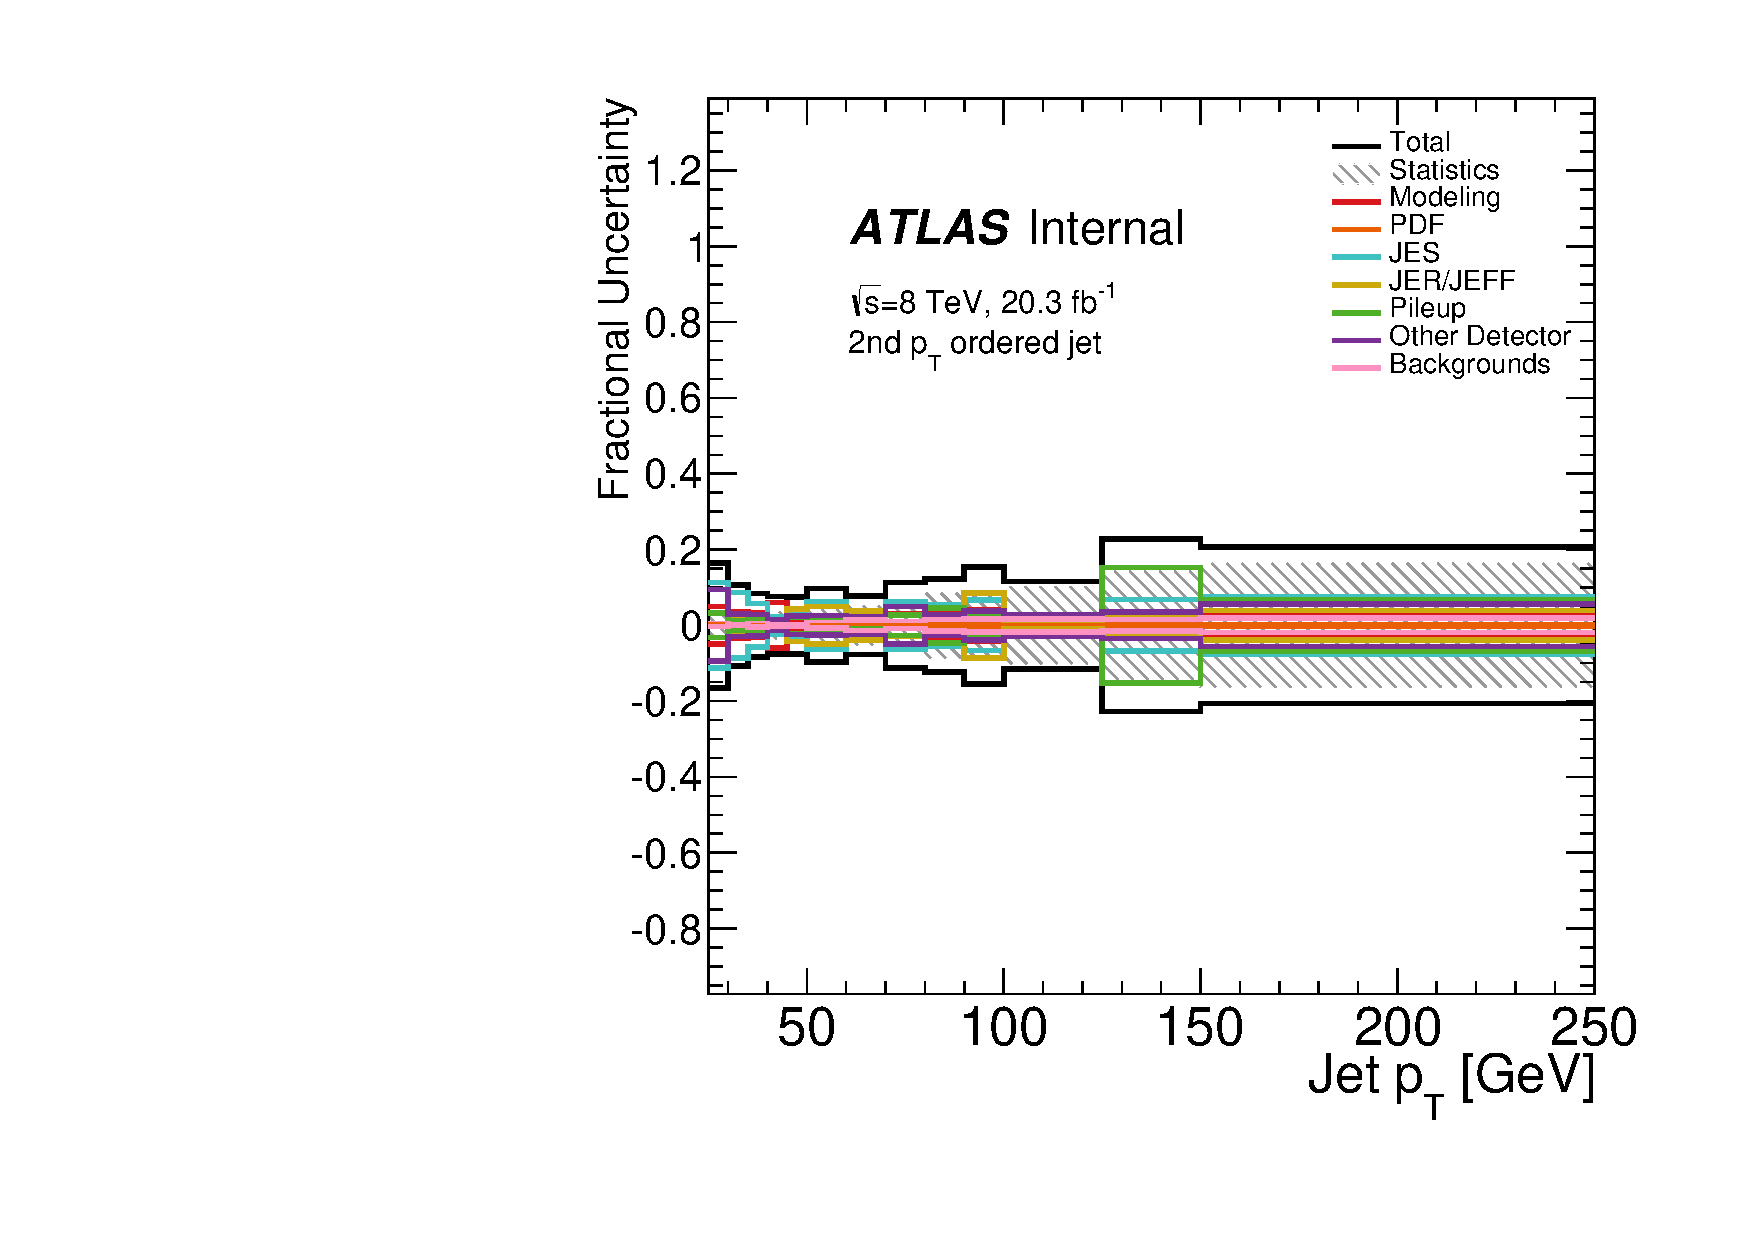
\includegraphics[width=\textwidth]{fig/UnfoldSys/Jet1.pdf}
\end{subfigure} \\
~
\begin{subfigure}[]{0.45\textwidth}
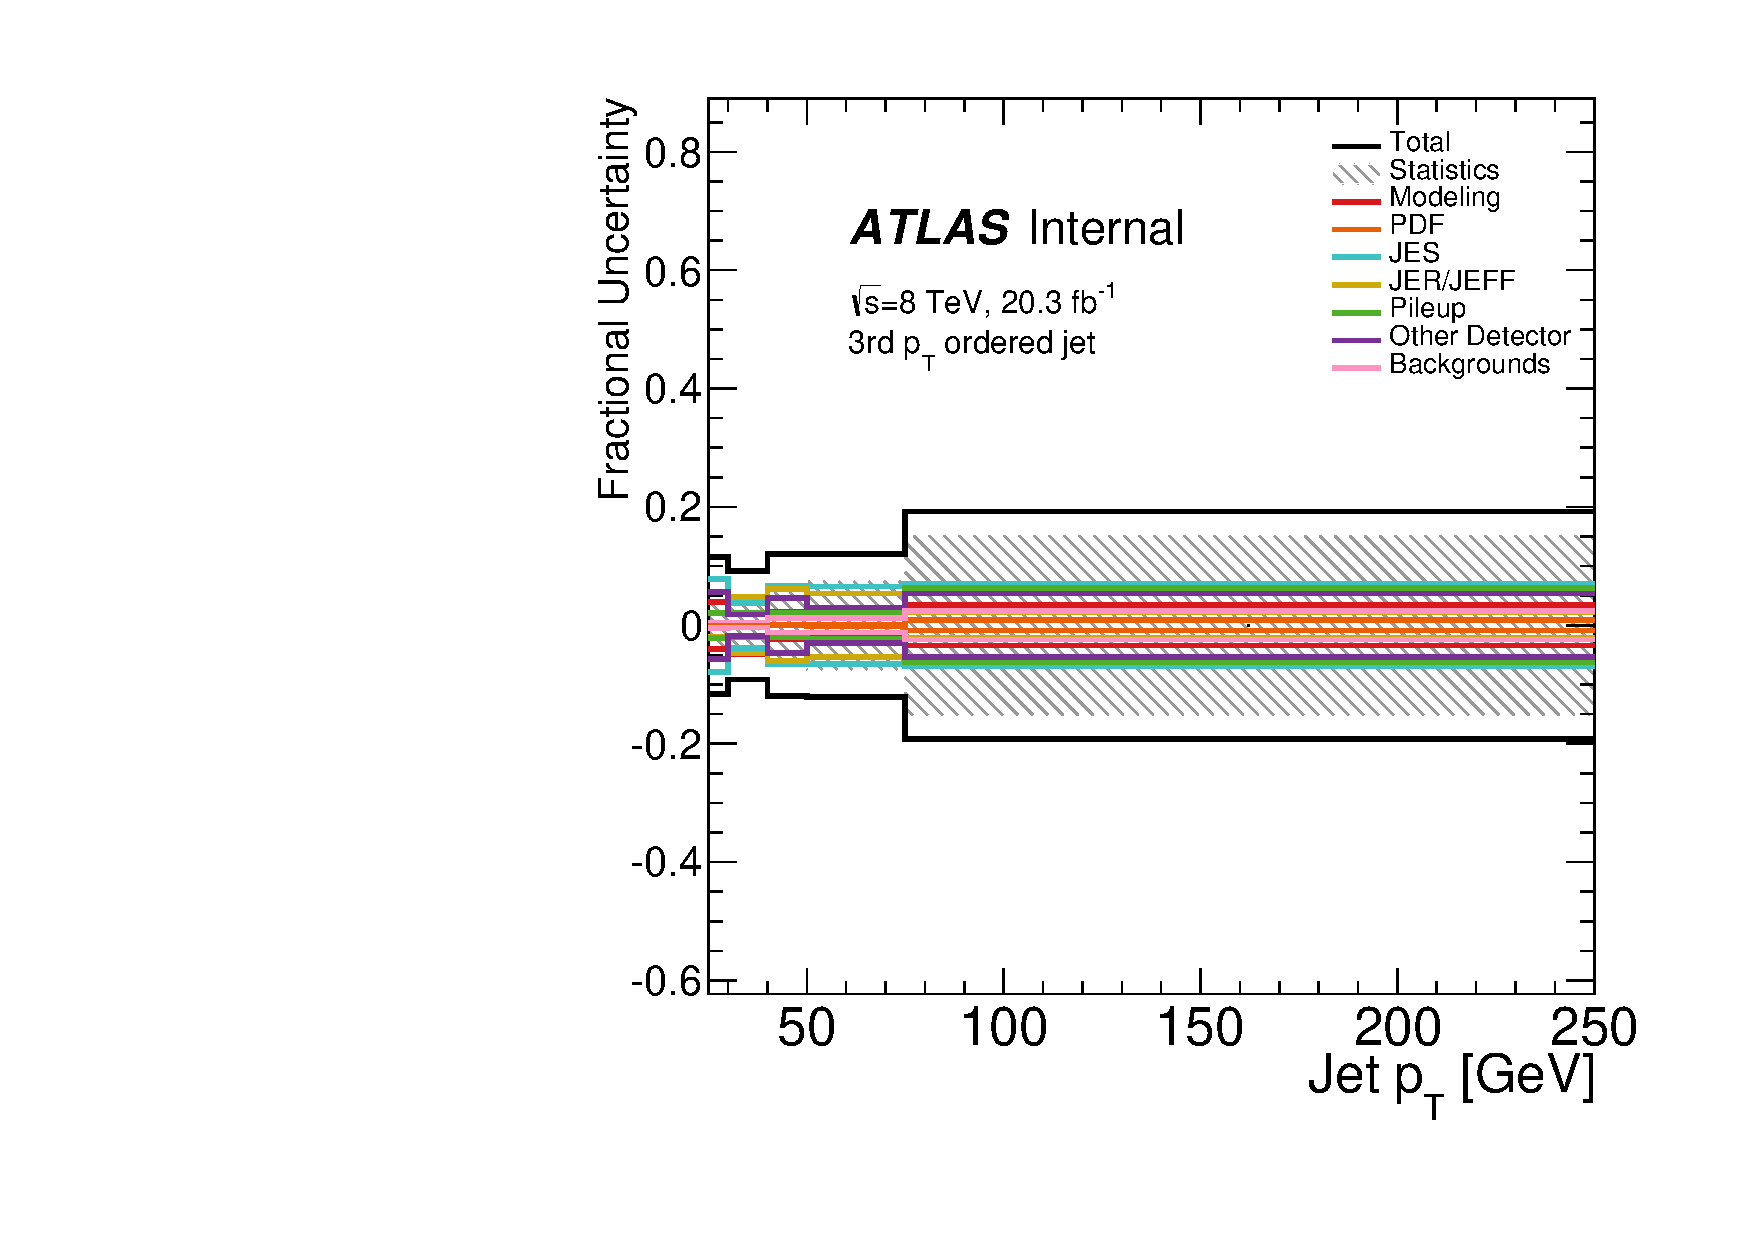
\includegraphics[width=\textwidth]{fig/UnfoldSys/Jet2.pdf}
\end{subfigure}
~
\begin{subfigure}[]{0.45\textwidth}
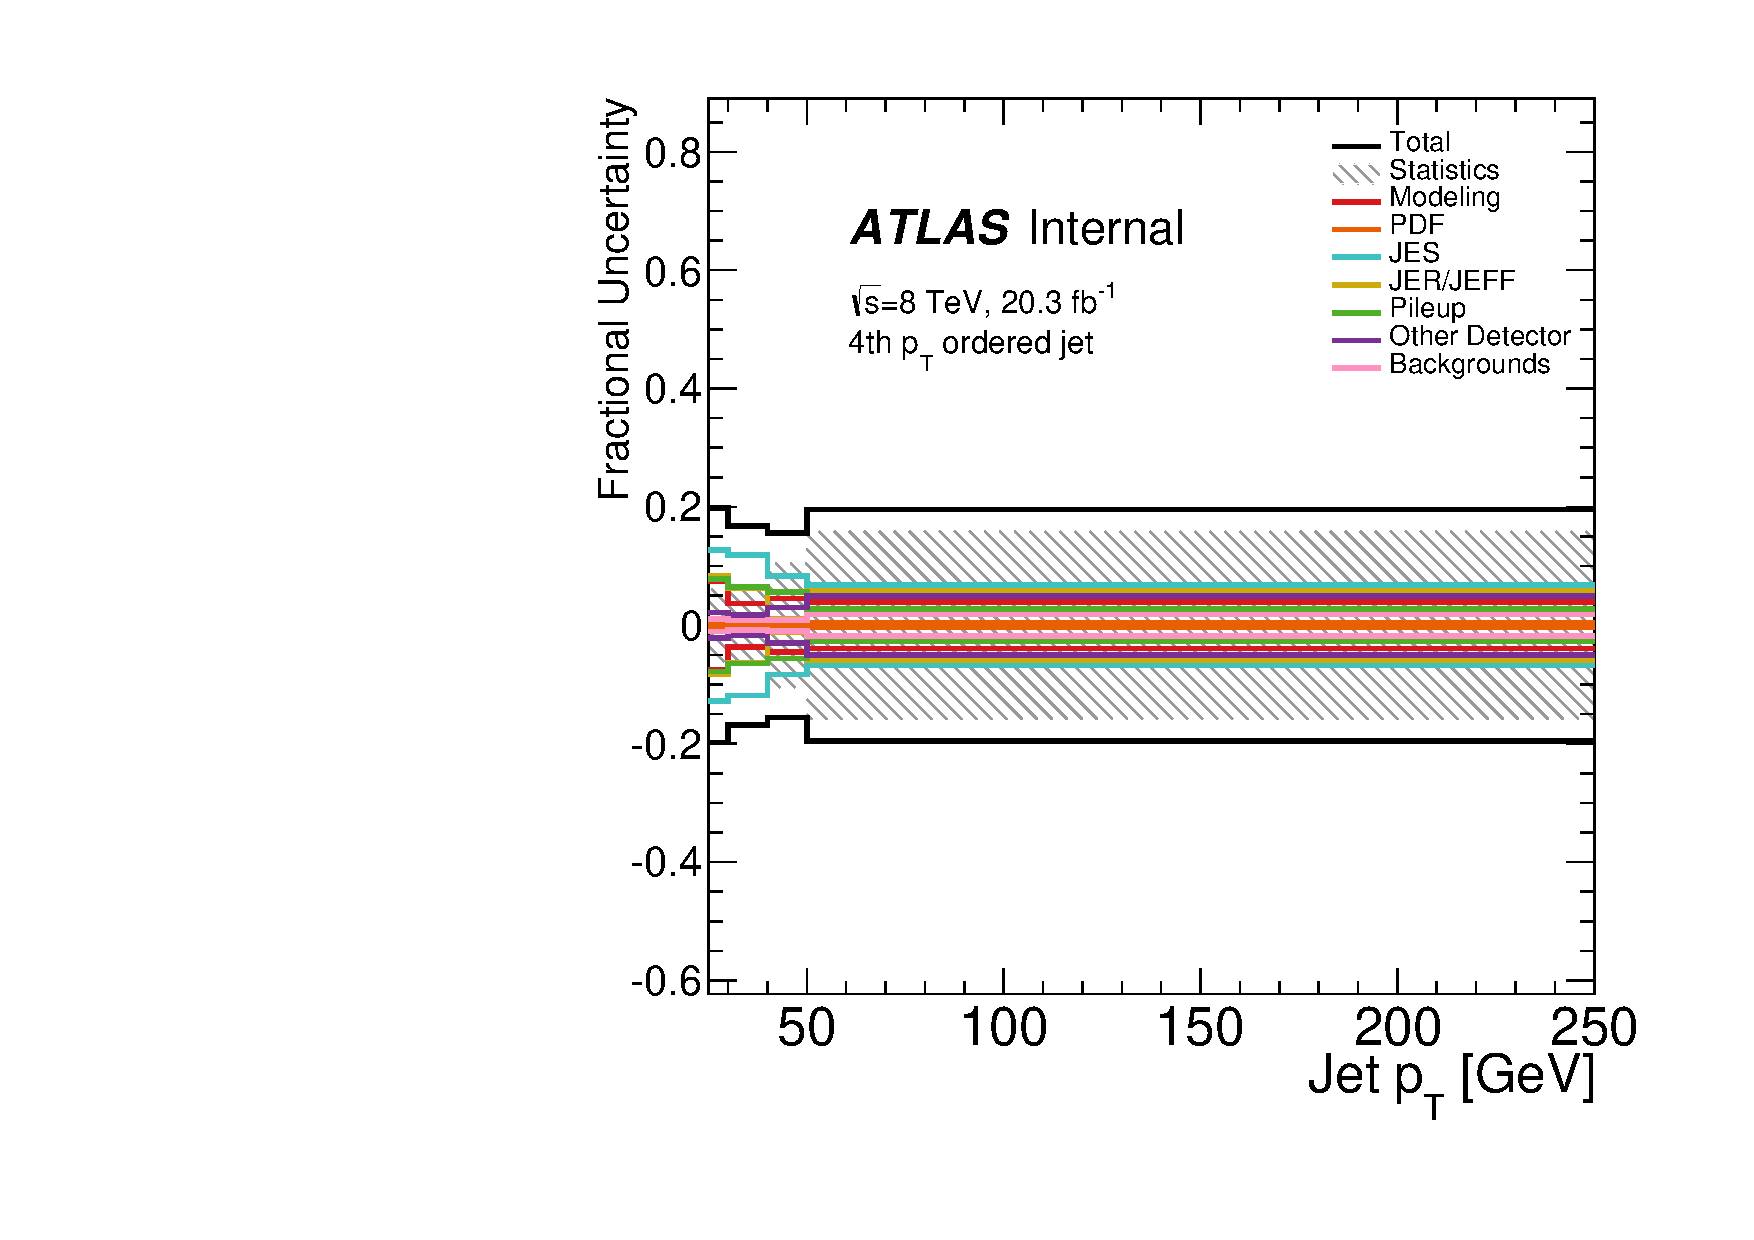
\includegraphics[width=\textwidth]{fig/UnfoldSys/Jet3.pdf}
\end{subfigure}
~
\caption{Sum of systematic uncertainties due to detector modeling. The ratio of the simulated extra jets reconstructed with each systematic variation is taken with respect to the nominal. The band shows the data statistical uncertainty for reference.}
\label{fig:SmoothSys}
\end{figure}

\begin{figure}
\begin{subfigure}[]{0.45\textwidth}
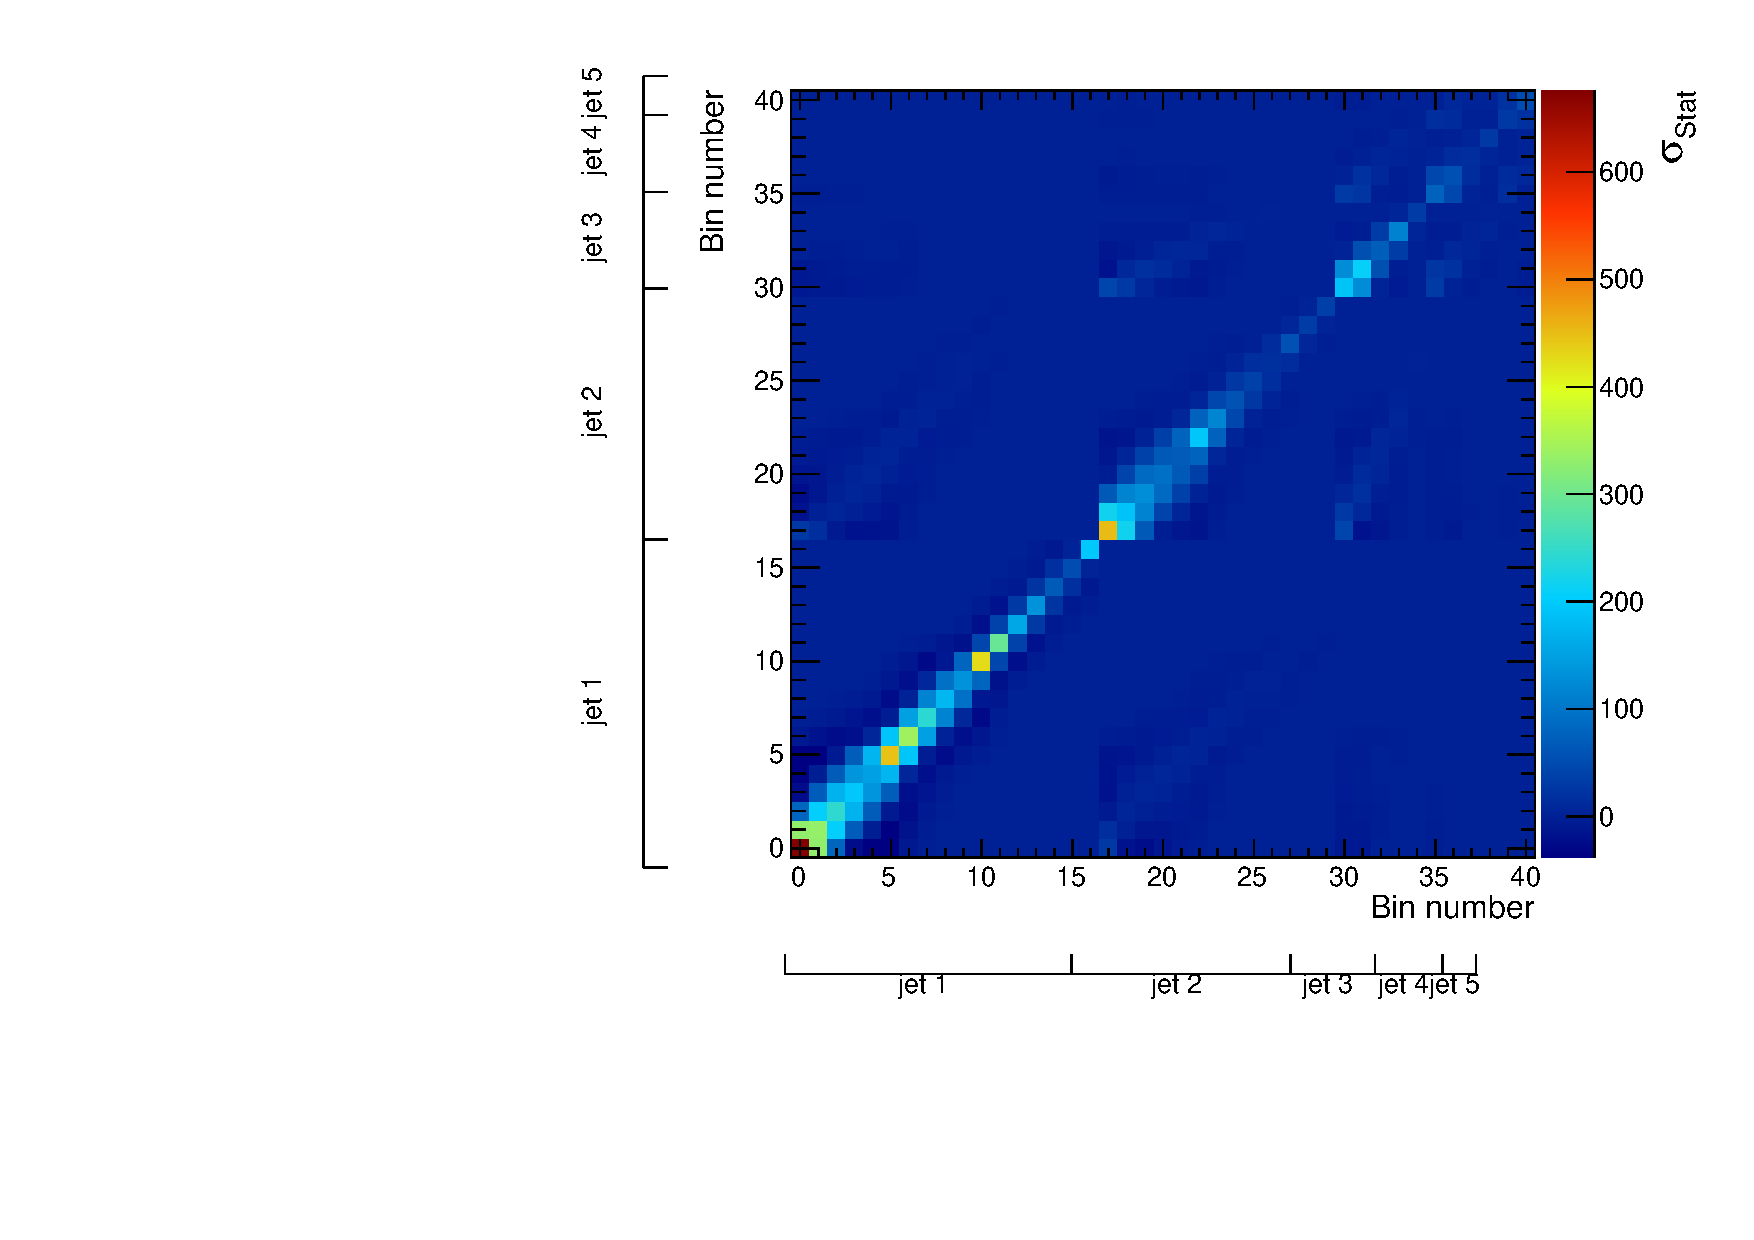
\includegraphics[width=\textwidth]{fig/Cov/Stat.pdf}
\end{subfigure}
~
\begin{subfigure}[]{0.45\textwidth}
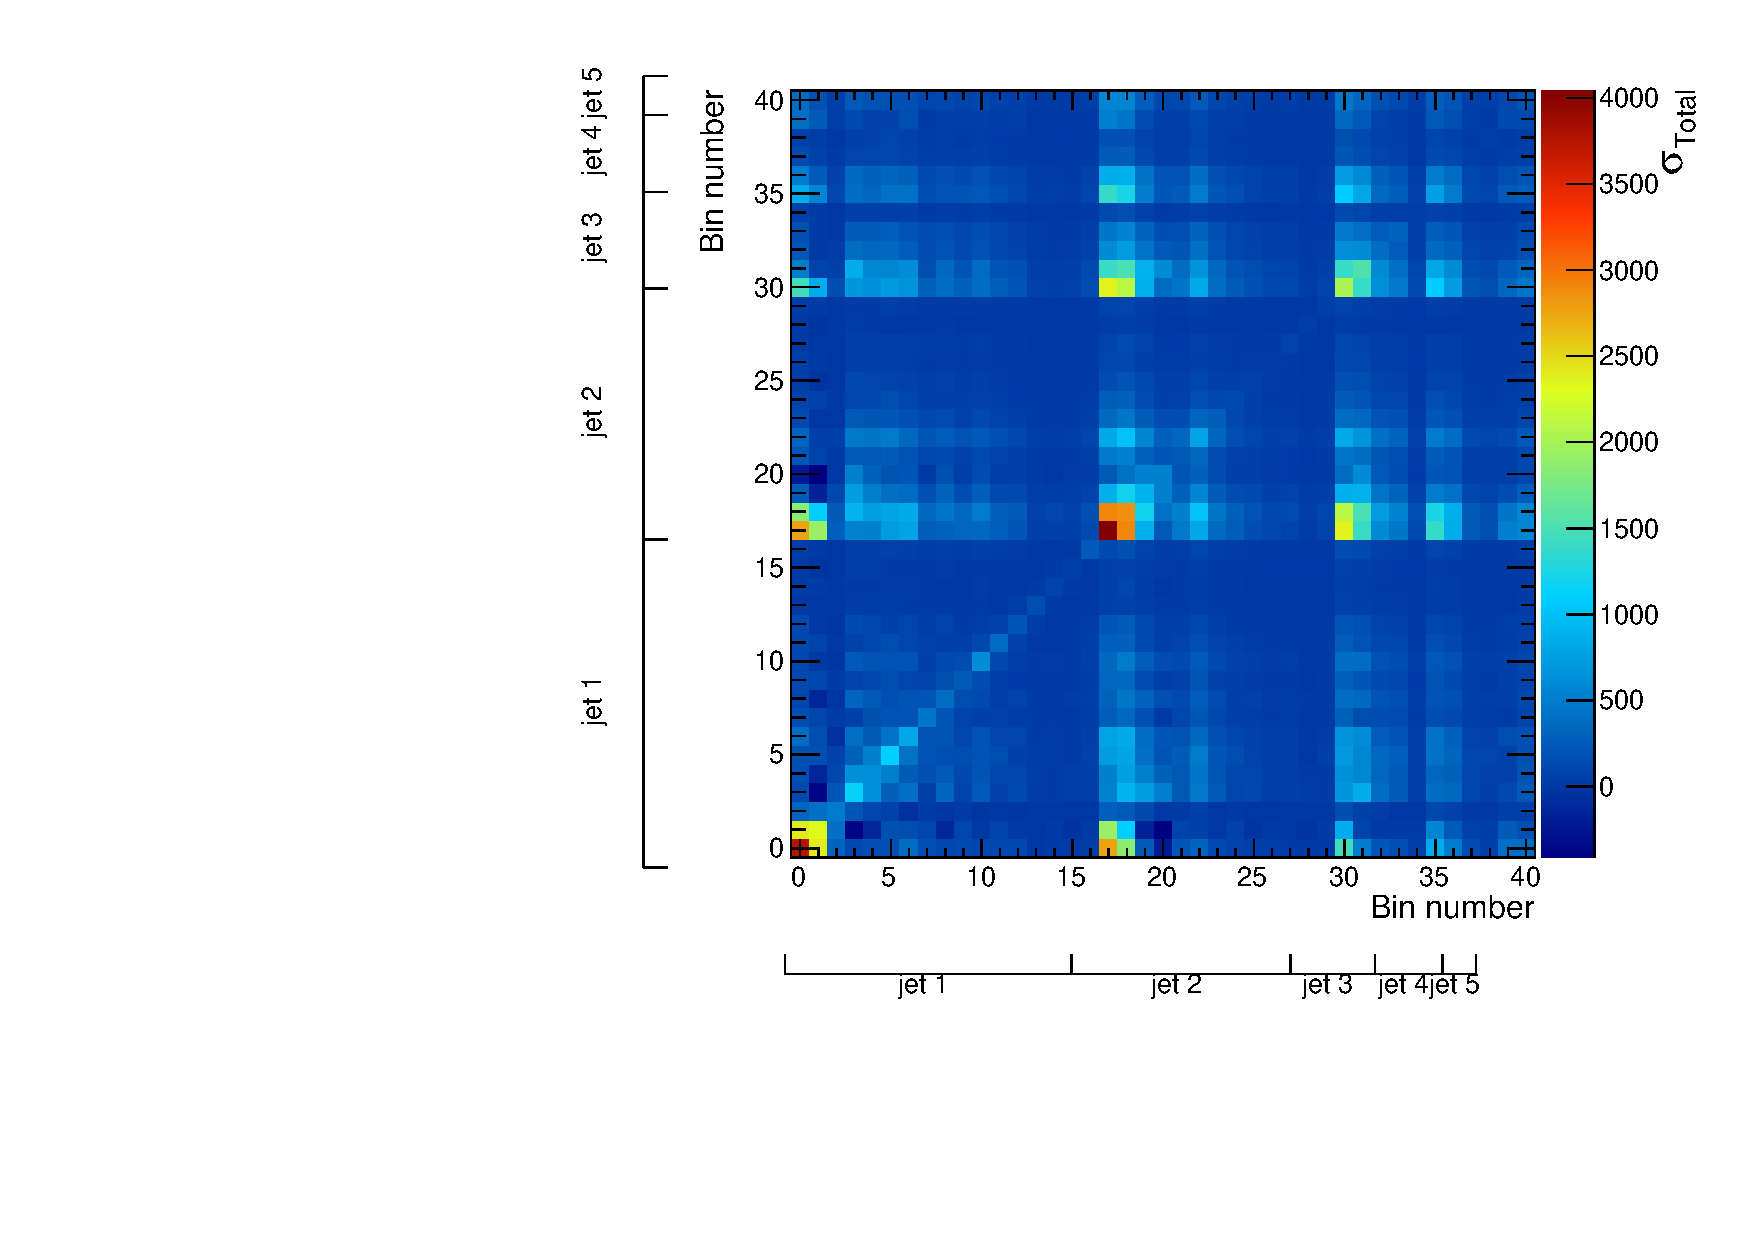
\includegraphics[width=\textwidth]{fig/Cov/Total.pdf}
\end{subfigure}
~
\caption{(a) The covariance matrix associated with the statistical uncertainty of the input spectrum returned from \texttt{ RooUnfold}. (b) The covariance matrix from all sources of uncertainty, obtained by adding the covariance matrices from all sources of systematic uncertainty to (a). This matrix is used to determine the \chisq\ agreement between generators and the fully corrected data.}
\label{fig:cov}
\end{figure}



